\section{Estimating parameter E for reaction 3 for 53$\%$ ozone }

The results displayed in this section are for the uncertainty involved in the calculation of flamespeed depending only on one parameter i.e the activation energy for the fall off reaction in the ozone mechanism. The percentage of ozone is 53 percent.The results are dispalyed in two section. In first section, The sample size for surrogate is changed and it is clear that for varying sized the map point of the resulting pdf does not change greatly. The surrogate are constructed using linear interpolation function. The initial guess for the map point is calculated using nelder mead optimization technique. After supplying initial guess over large domain it is found that the map point is the same no matter where we start our guess. 
\bigskip

\subsubsection{Different surrogate sizes }

\noindent Here the surrogate size is defined as $sample size*1$ vector. The flamespeed is calculated for given samples in the domain ( 0 to 34.76). Other values are calculated as linear interpolation of these points. In this analysis, constant raw chain size of 500,000 is taken. 
\subsubsection{Sample size (Surrogate size) 10 }
In this section we calculated flamespeed values for 10 different points in the domain and the remaining values are linear combination of these 10 points.  
\begin{figure}[H]
  
  \centering
   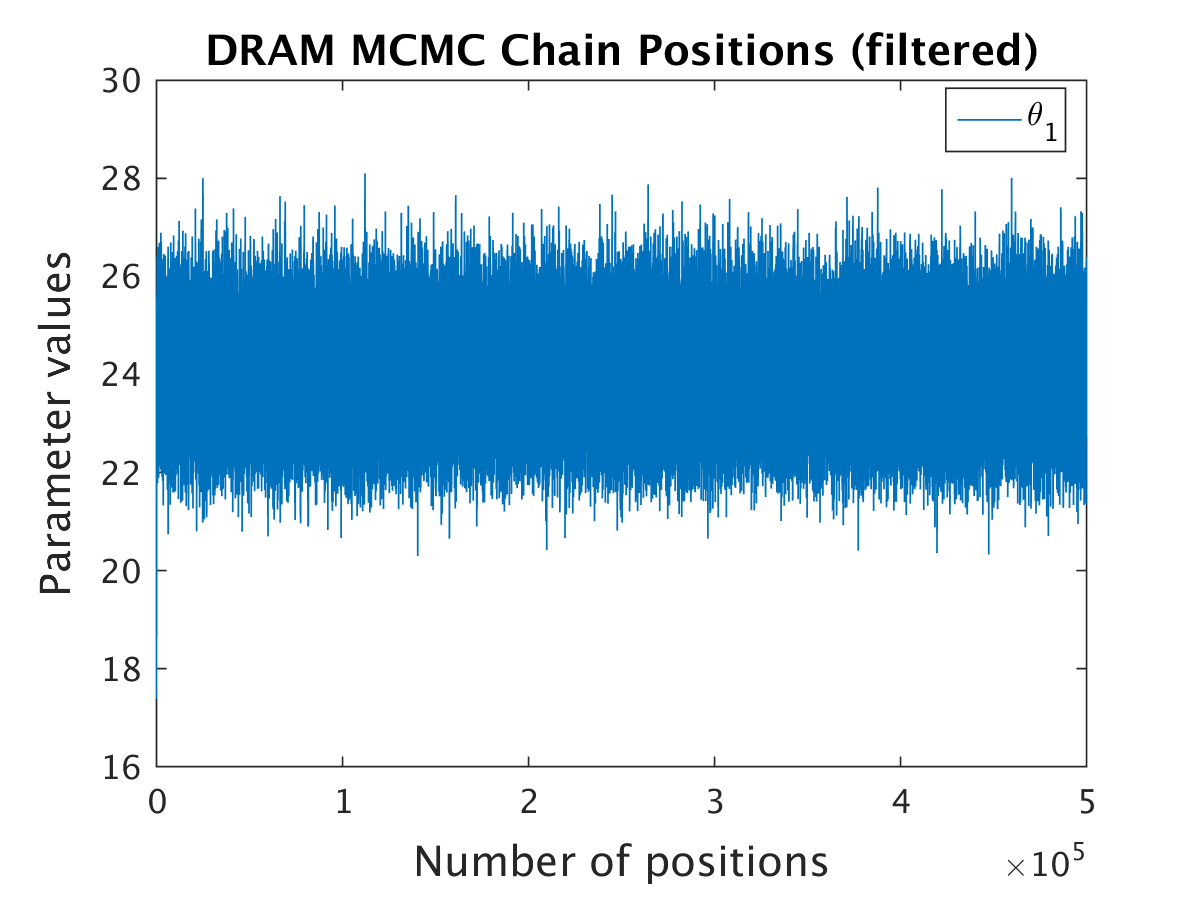
\includegraphics[scale=0.75]{100_results/outputData_10/simple_ip_chain_pos_filt}
   \caption{MCMC chain position }
\end{figure}


\begin{figure}[H]
  
  \centering
   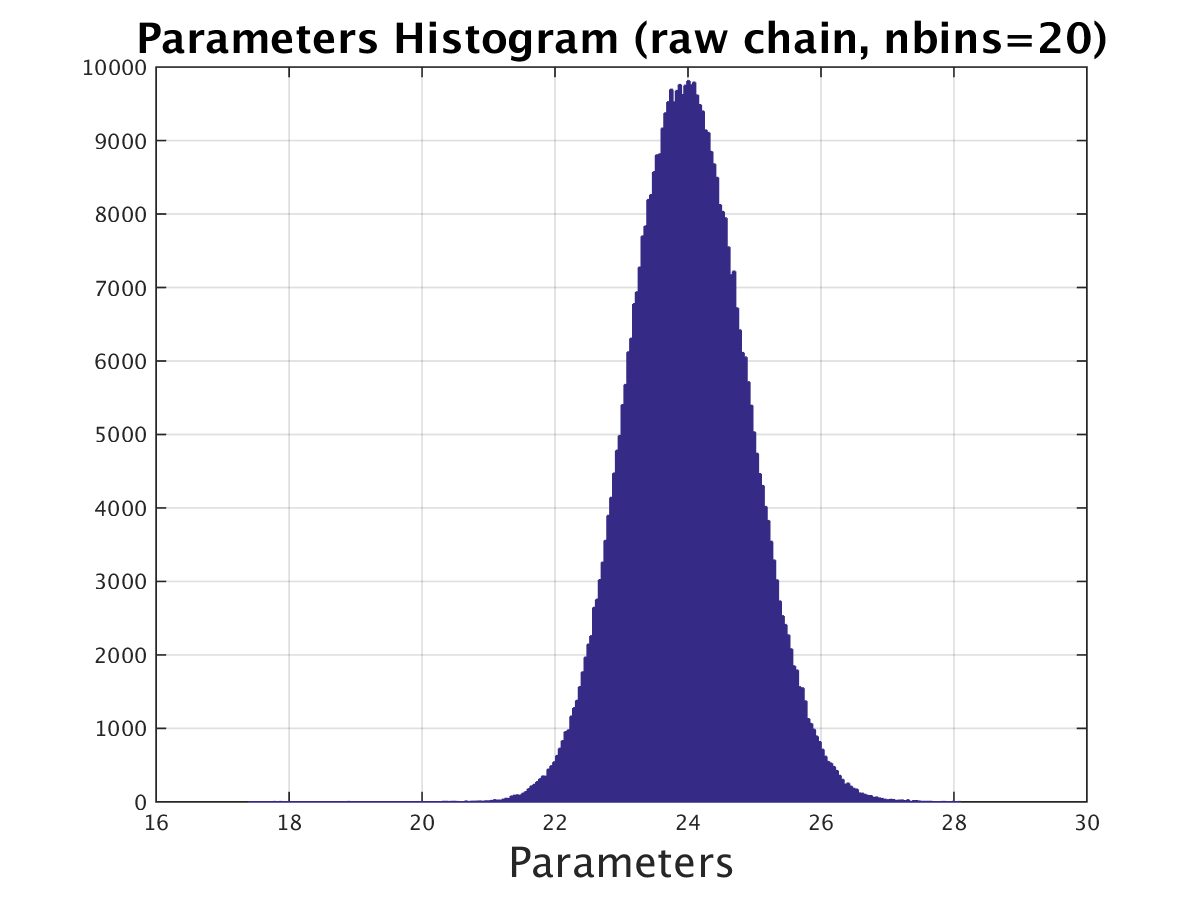
\includegraphics[scale=0.75]{100_results/outputData_10/simple_ip_hist_raw}
   \caption{Histogram}
\end{figure}



\begin{figure}[H]
  
  \centering
   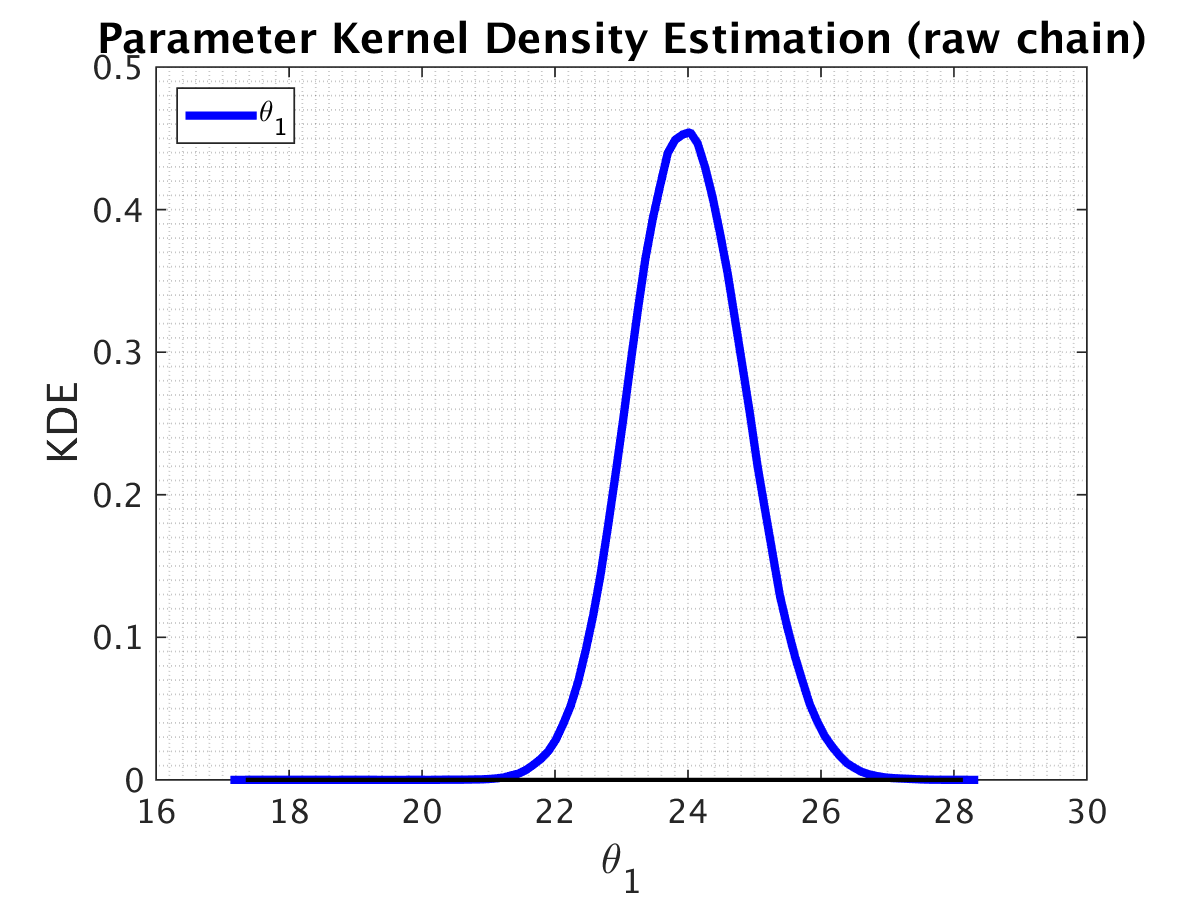
\includegraphics[scale=0.75]{100_results/outputData_10/simple_ip_kde_raw}
   \caption{ KDE }
\end{figure}

\begin{figure}[H]
  
  \centering
   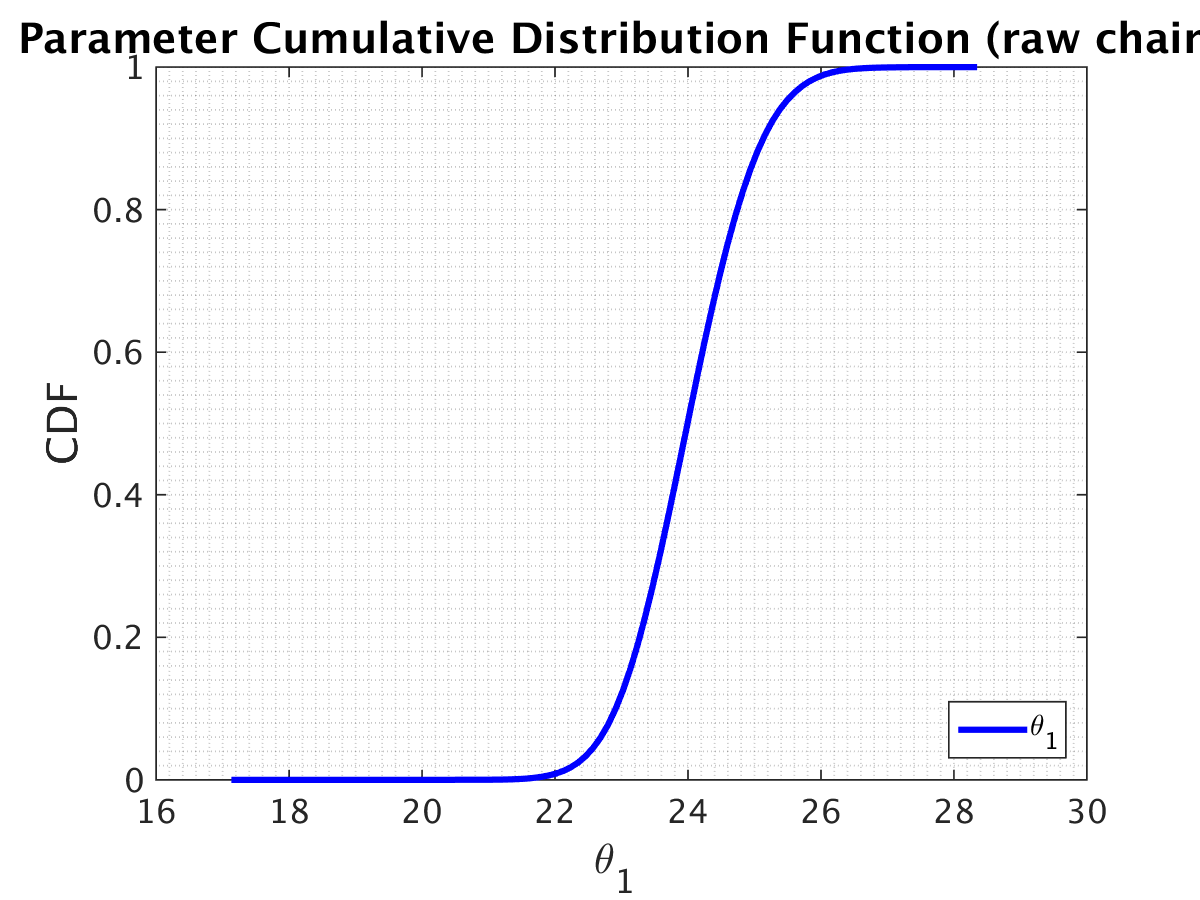
\includegraphics[scale=0.75]{100_results/outputData_10/simple_ip_cdf_raw}
   \caption{CDF function for Parameter }
\end{figure}



\begin{figure}[H]
  
  \centering
   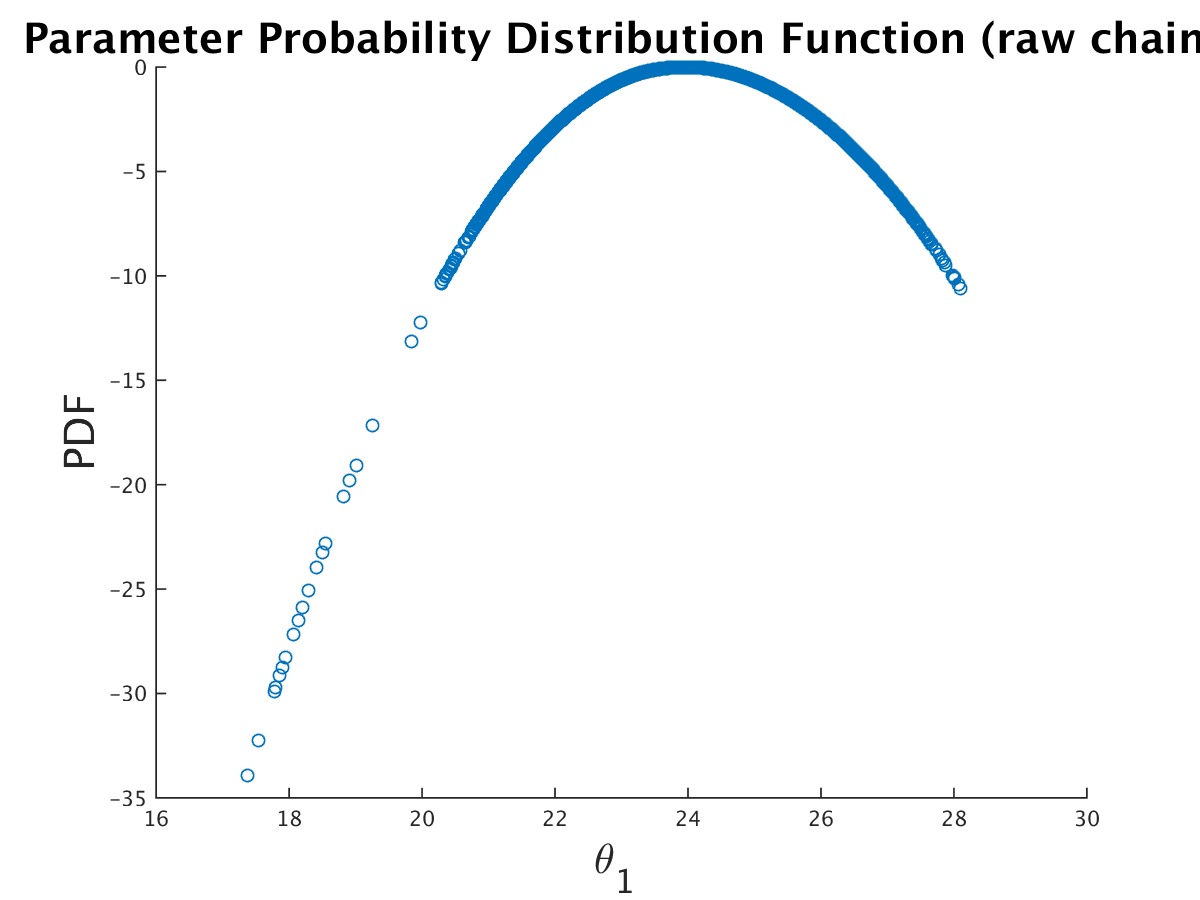
\includegraphics[scale=0.75]{100_results/outputData_10/ip_logLike_unified}
   \caption{PDF function for Parameter }
\end{figure}



\subsubsection{Sample size (Surrogate size) 20 }

In this section we calculated flamespeed values for 20 different points in the domain and the remaining values are linear combination of these 20. We can see that our results do not change drastically. 

\begin{figure}[H]
  
  \centering
   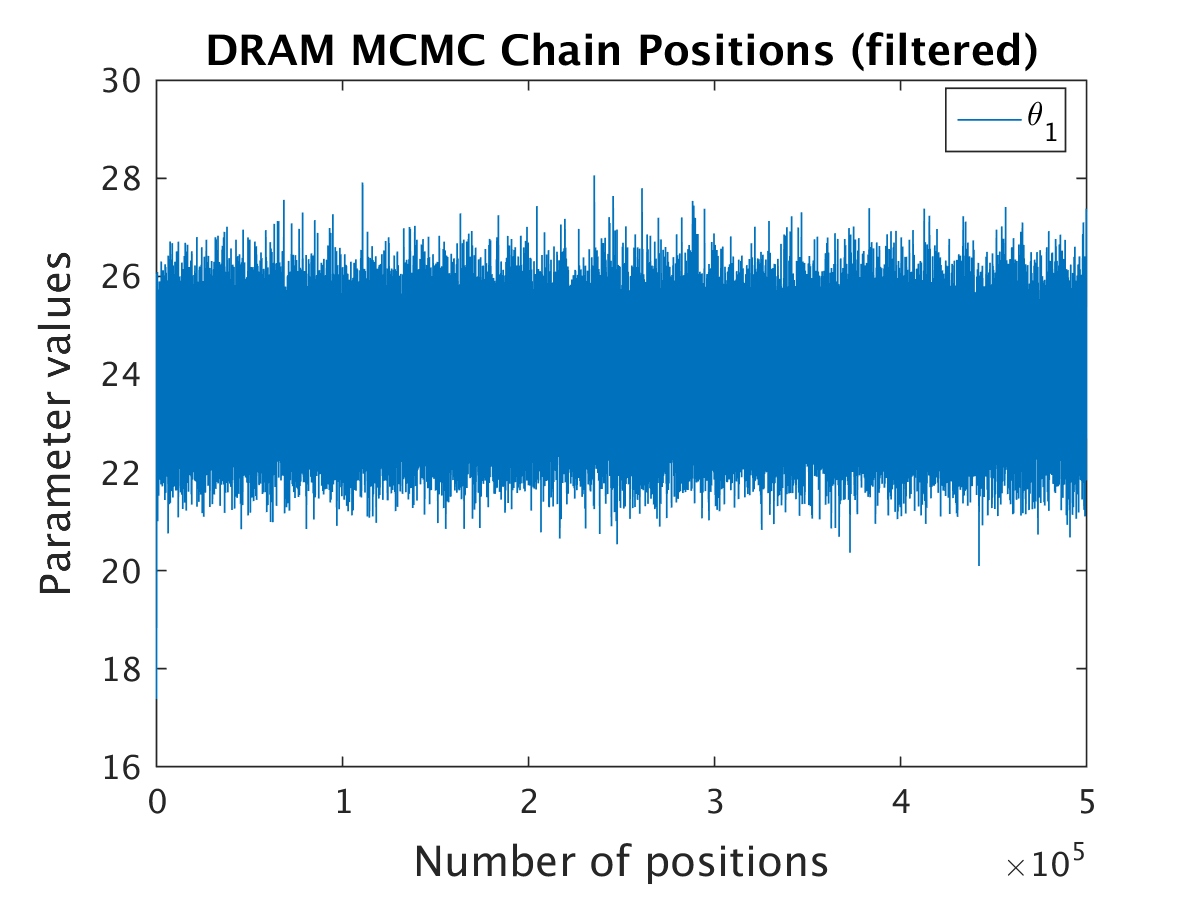
\includegraphics[scale=0.75]{100_results/outputData_20/simple_ip_chain_pos_filt}
   \caption{MCMC chain position }
\end{figure}


\begin{figure}[H]
  
  \centering
   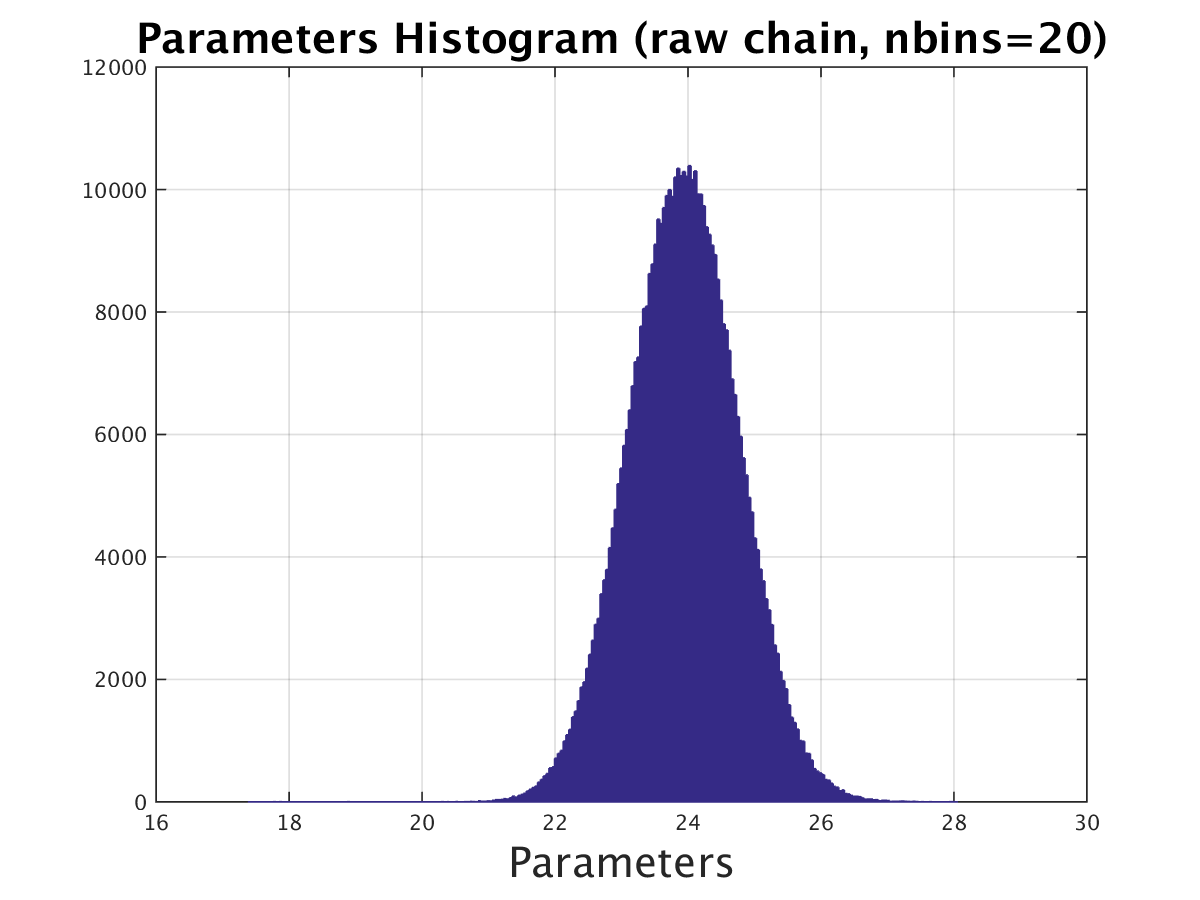
\includegraphics[scale=0.75]{100_results/outputData_20/simple_ip_hist_raw}
   \caption{Histogram}
\end{figure}



\begin{figure}[H]
  
  \centering
   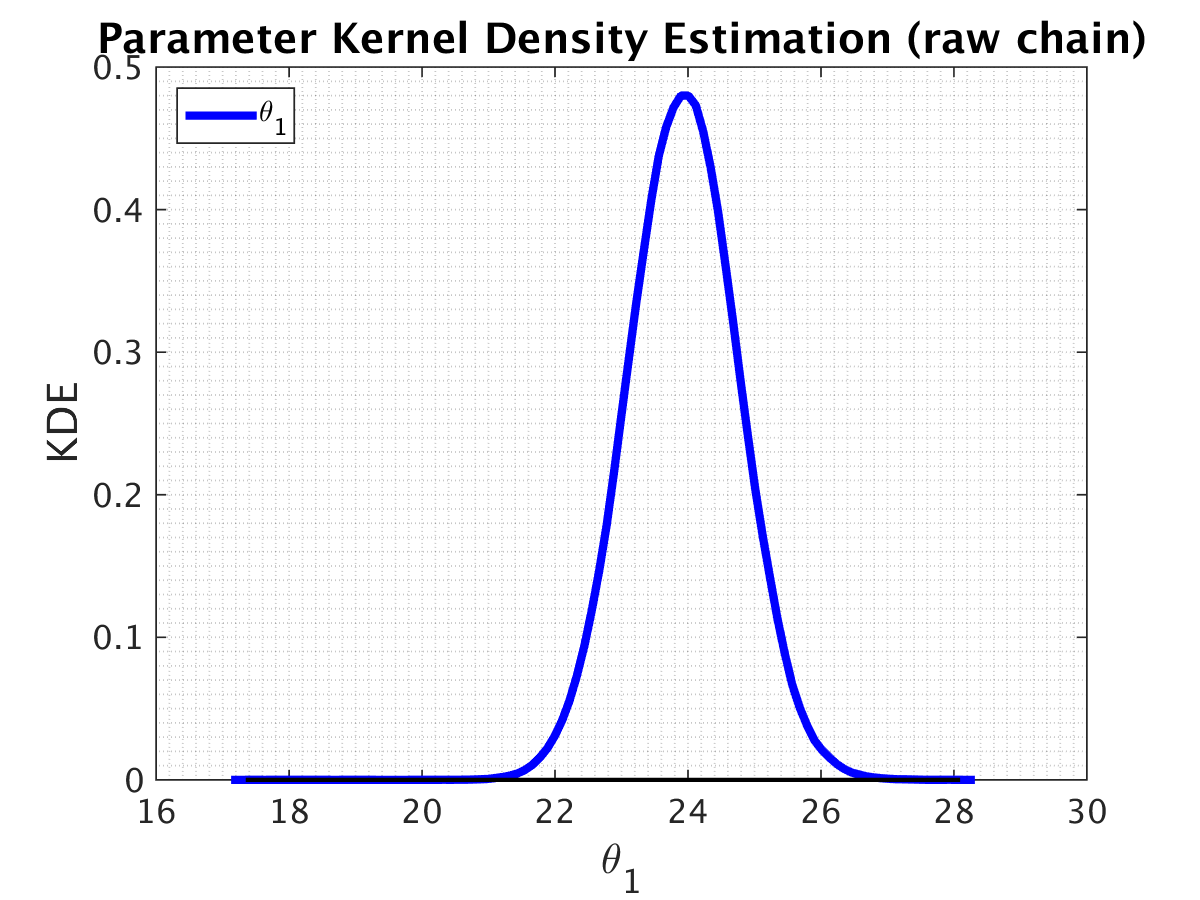
\includegraphics[scale=0.75]{100_results/outputData_20/simple_ip_kde_raw}
   \caption{ KDE }
\end{figure}

\begin{figure}[H]
  
  \centering
   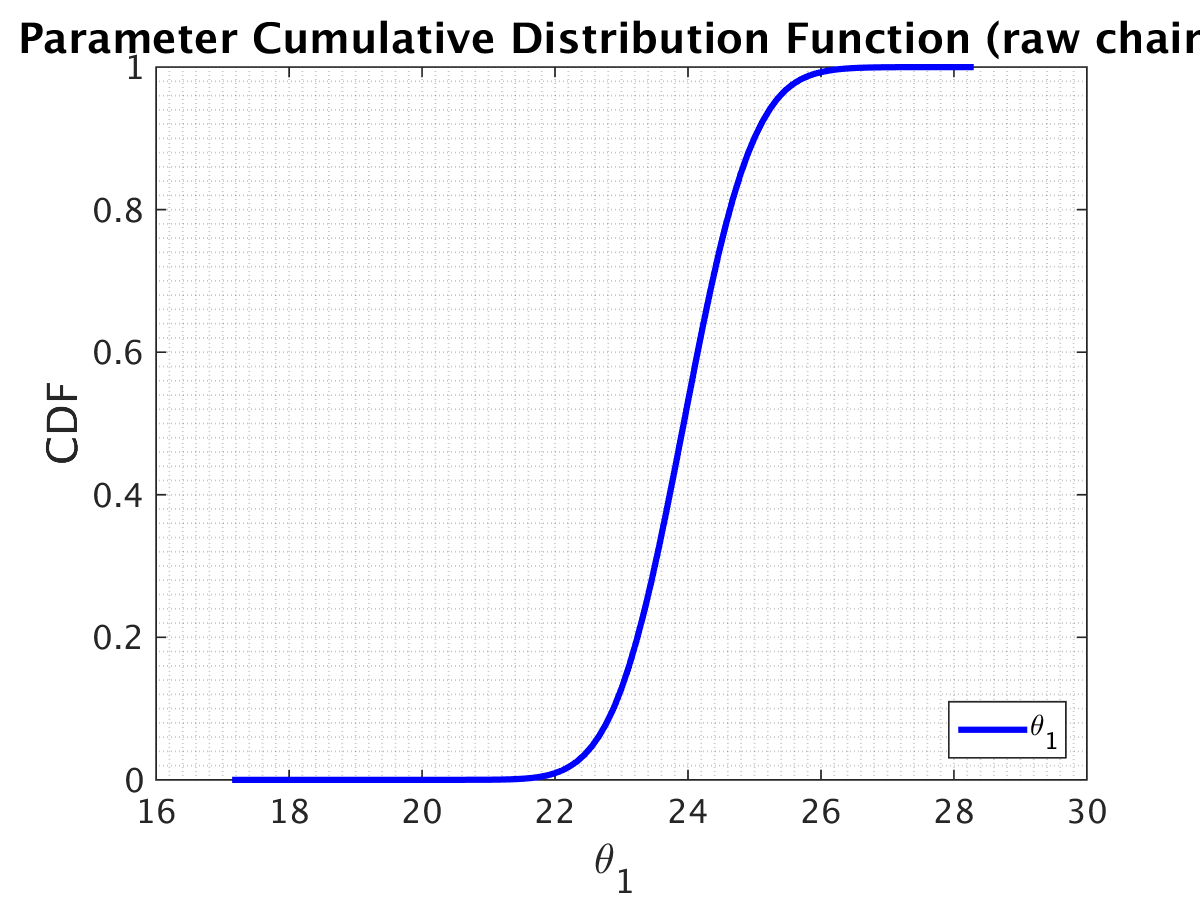
\includegraphics[scale=0.75]{100_results/outputData_20/simple_ip_cdf_raw}
   \caption{CDF function for Parameter }
\end{figure}



\begin{figure}[H]
  
  \centering
   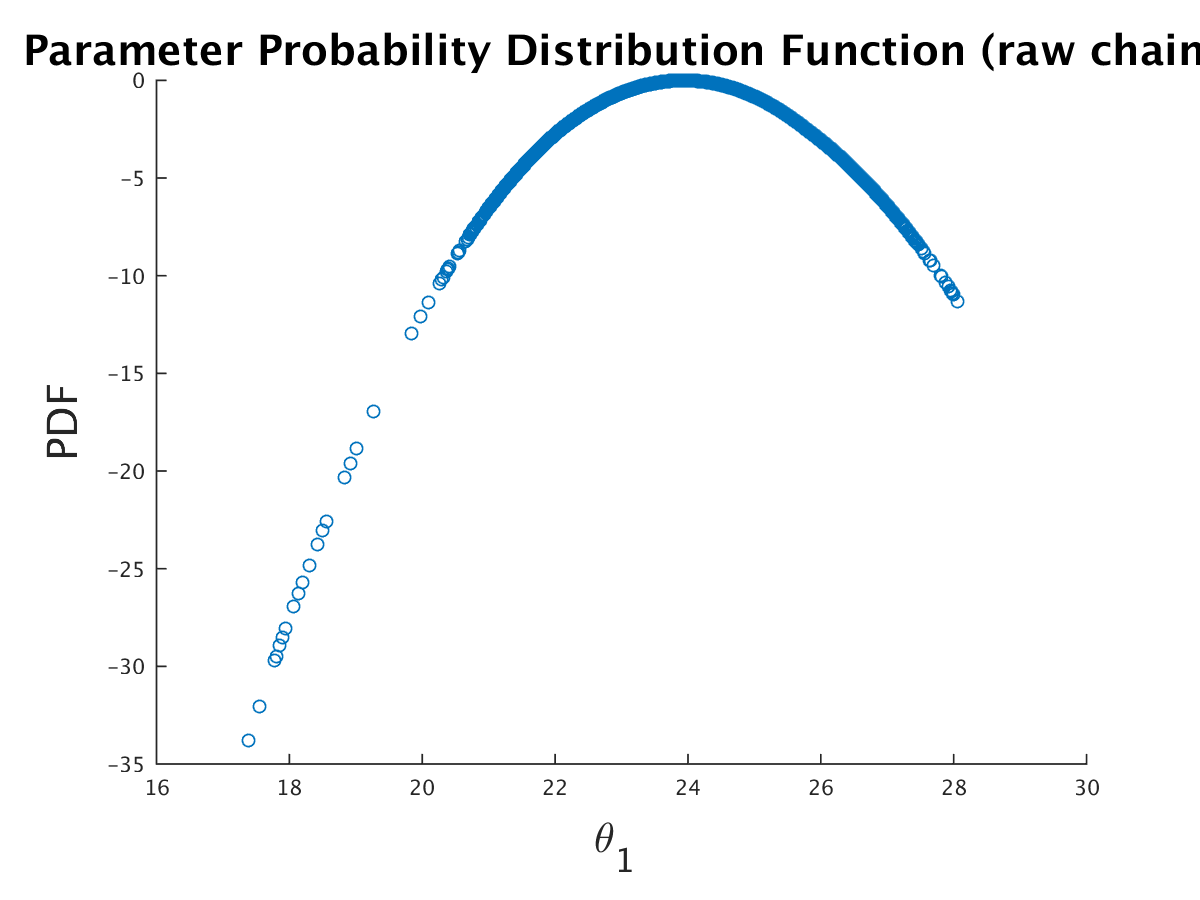
\includegraphics[scale=0.75]{100_results/outputData_20/ip_logLike_unified}
   \caption{PDF function for Parameter }
\end{figure}


\subsubsection{Sample size (Surrogate size) 50 }


In this section we calculated flamespeed values for 50 points in the domain 
\begin{figure}[H]
  
  \centering
   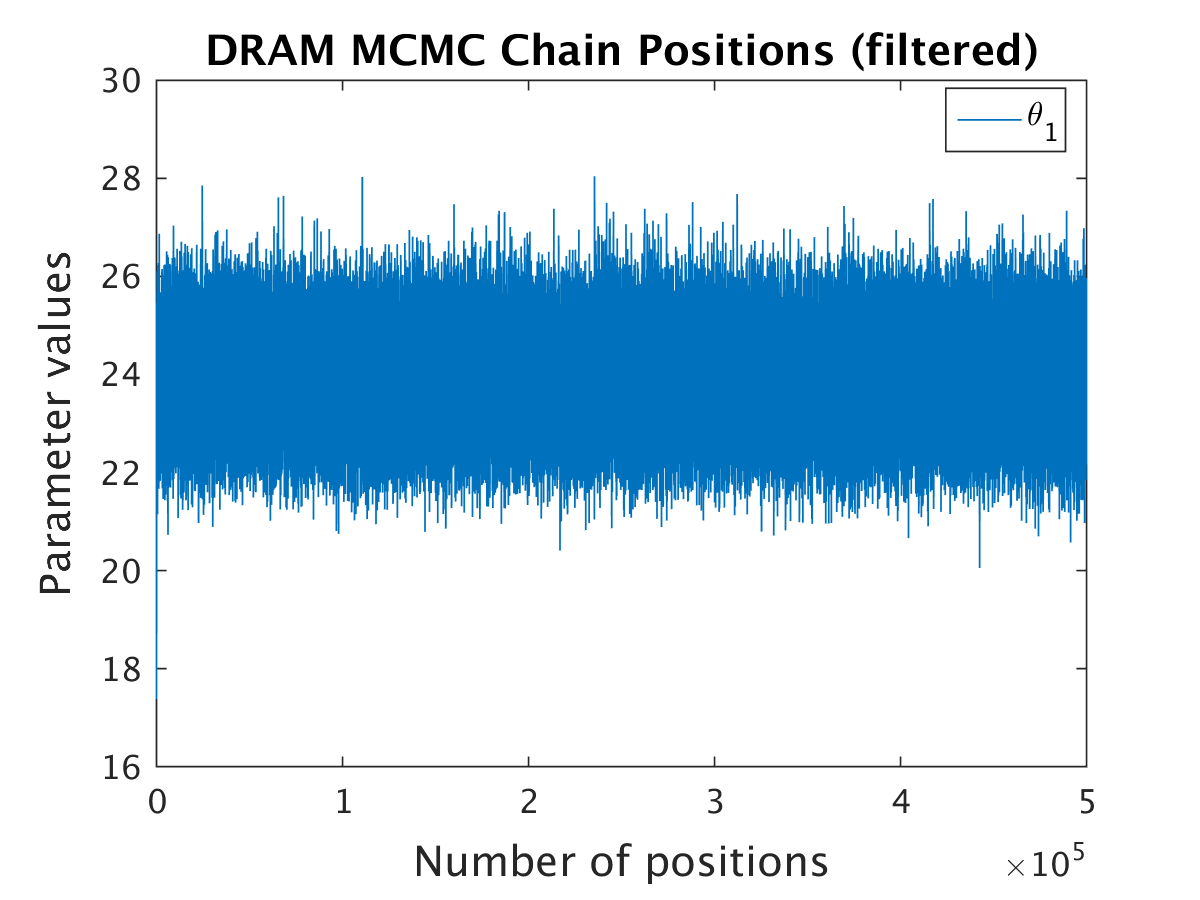
\includegraphics[scale=0.75]{100_results/outputData_50/simple_ip_chain_pos_filt}
   \caption{MCMC chain position }
\end{figure}


\begin{figure}[H]
  
  \centering
   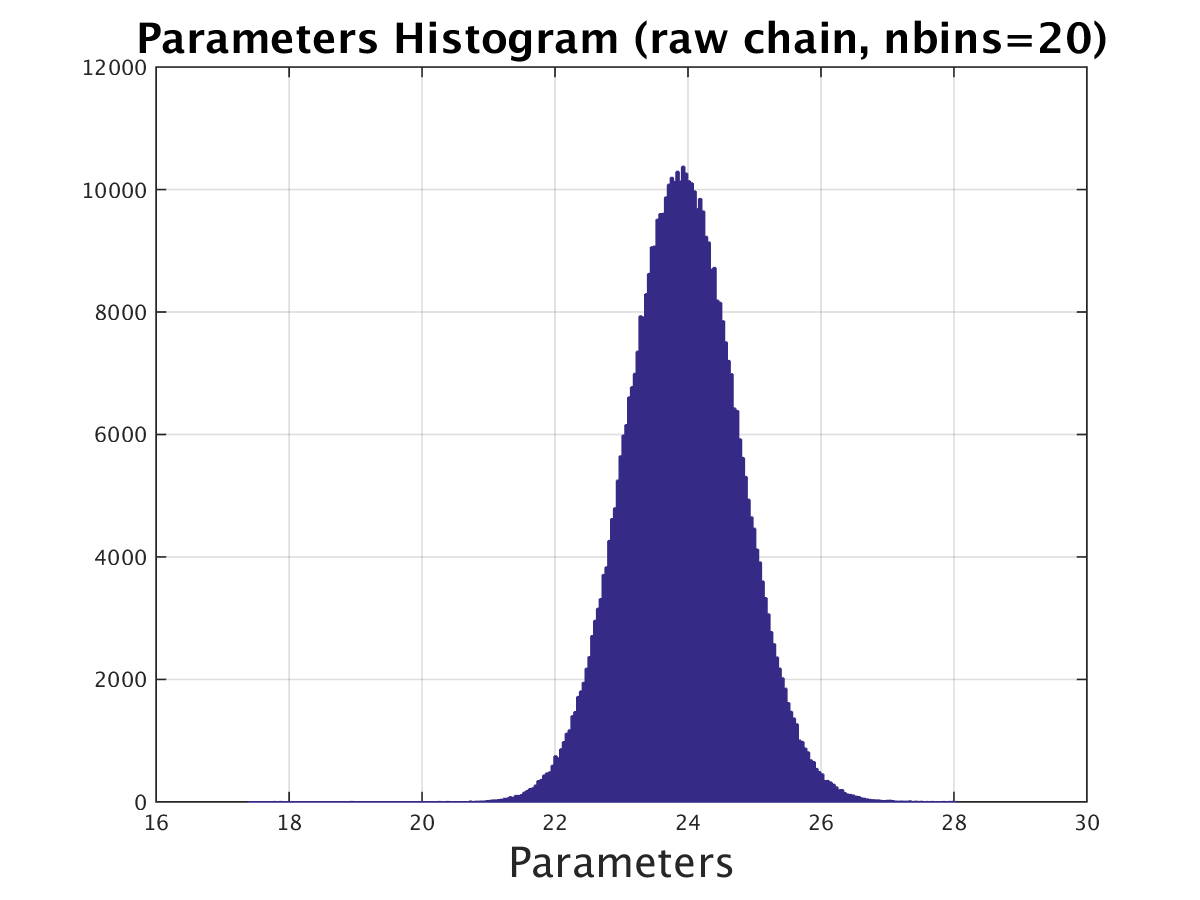
\includegraphics[scale=0.75]{100_results/outputData_50/simple_ip_hist_raw}
   \caption{Histogram}
\end{figure}



\begin{figure}[H]
  
  \centering
   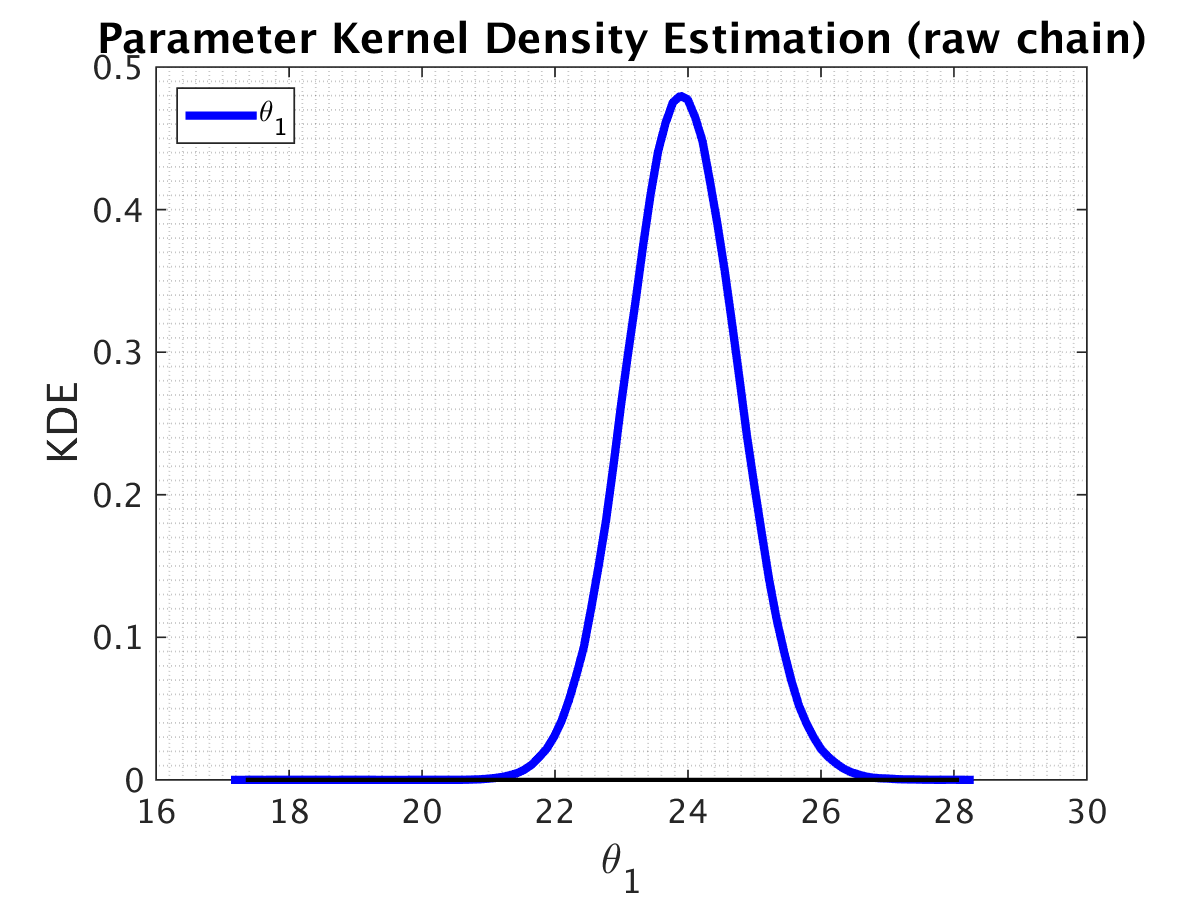
\includegraphics[scale=0.75]{100_results/outputData_50/simple_ip_kde_raw}
   \caption{ KDE }
\end{figure}

\begin{figure}[H]
  
  \centering
   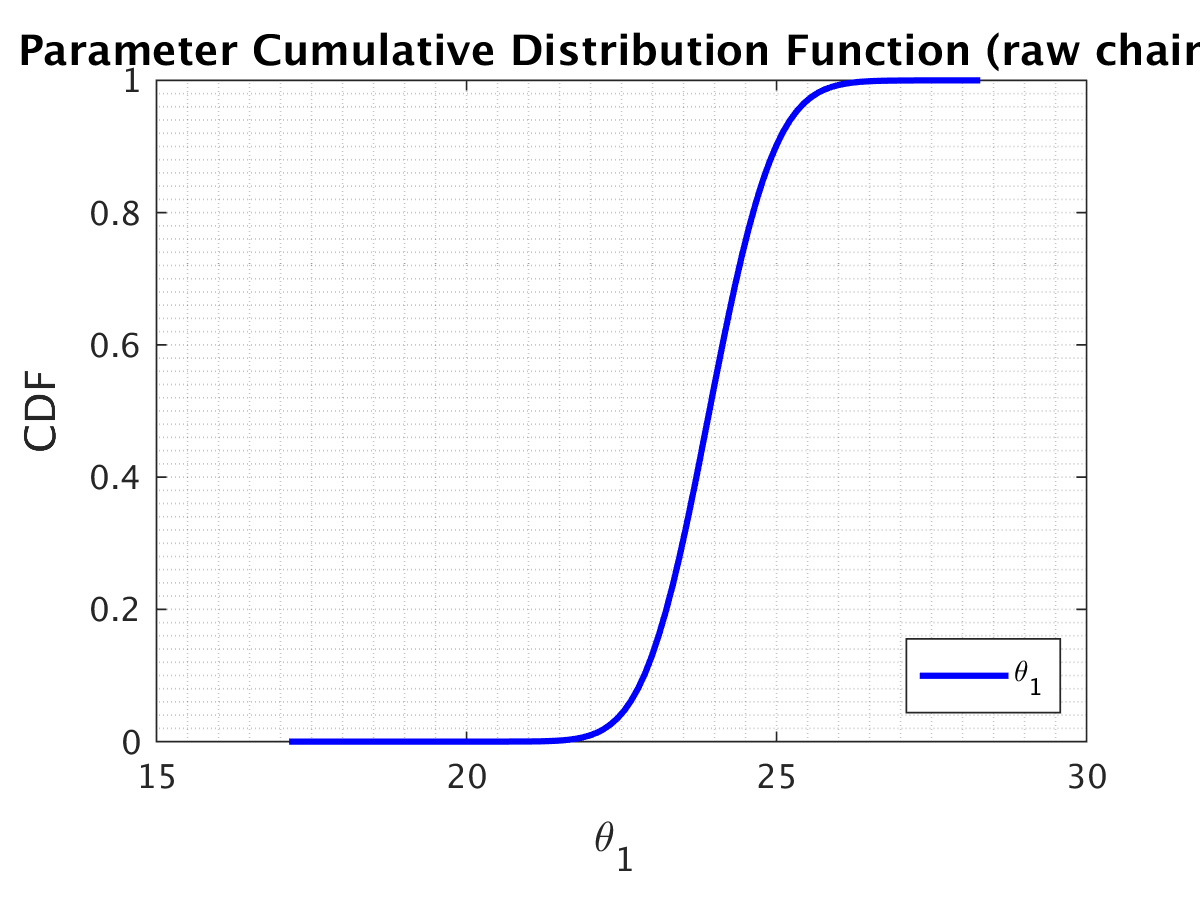
\includegraphics[scale=0.75]{100_results/outputData_50/simple_ip_cdf_raw}
   \caption{CDF function for Parameter }
\end{figure}



\begin{figure}[H]
  
  \centering
   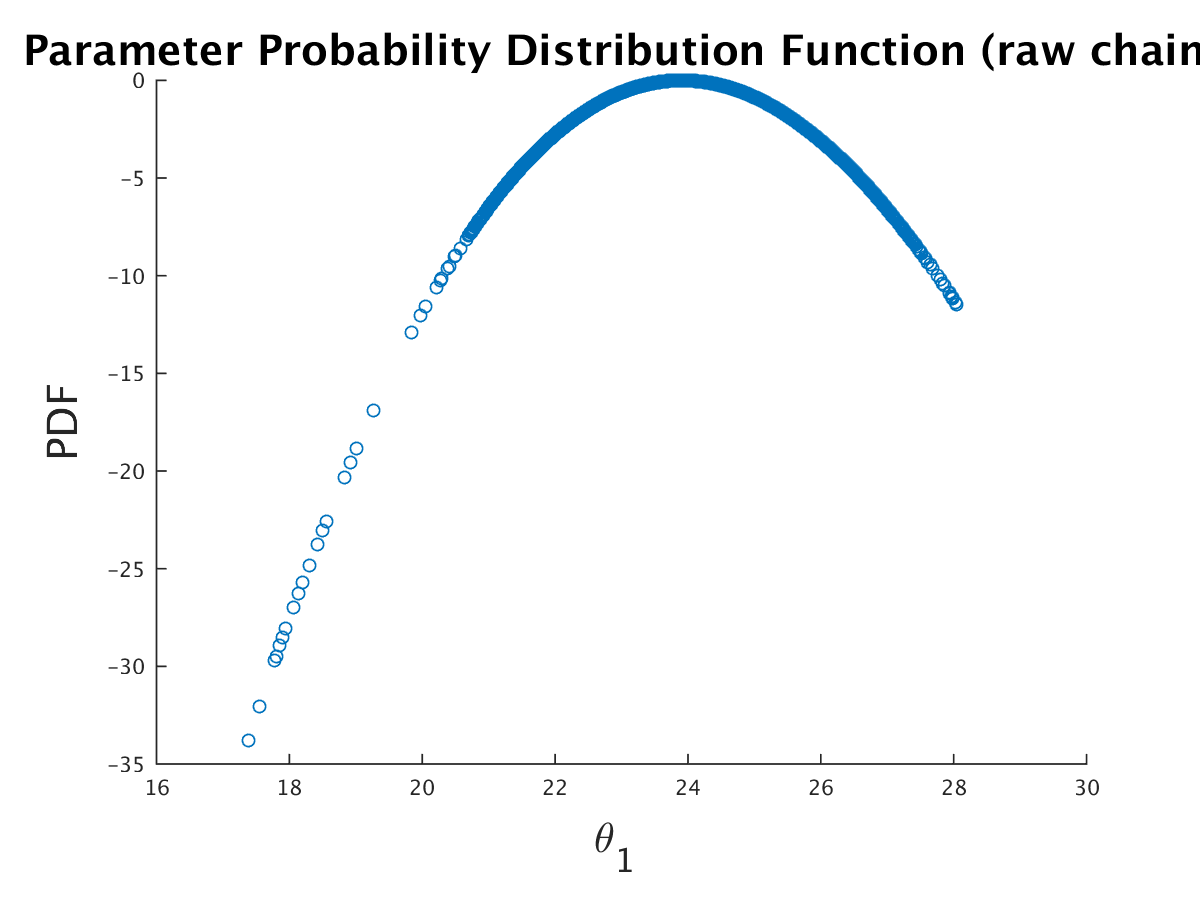
\includegraphics[scale=0.75]{100_results/outputData_50/ip_logLike_unified}
   \caption{PDF function for Parameter }
\end{figure}



\subsubsection{Sample size (Surrogate size) 100 }


In this section we calculated flamespeed values for 100 points in the domain 
\begin{figure}[H]
  
  \centering
   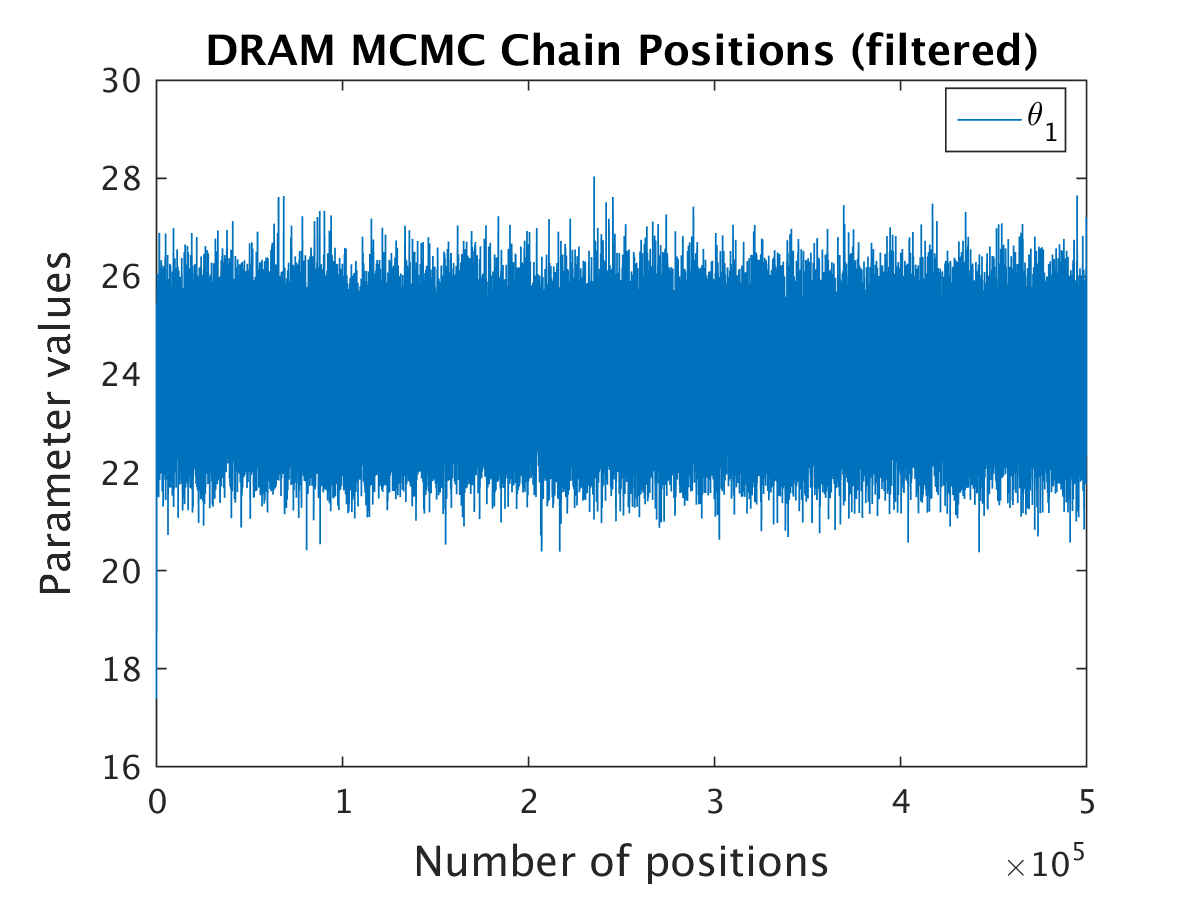
\includegraphics[scale=0.75]{100_results/outputData_100/simple_ip_chain_pos_filt}
   \caption{MCMC chain position }
\end{figure}
%
%
\begin{figure}[H]
  
  \centering
   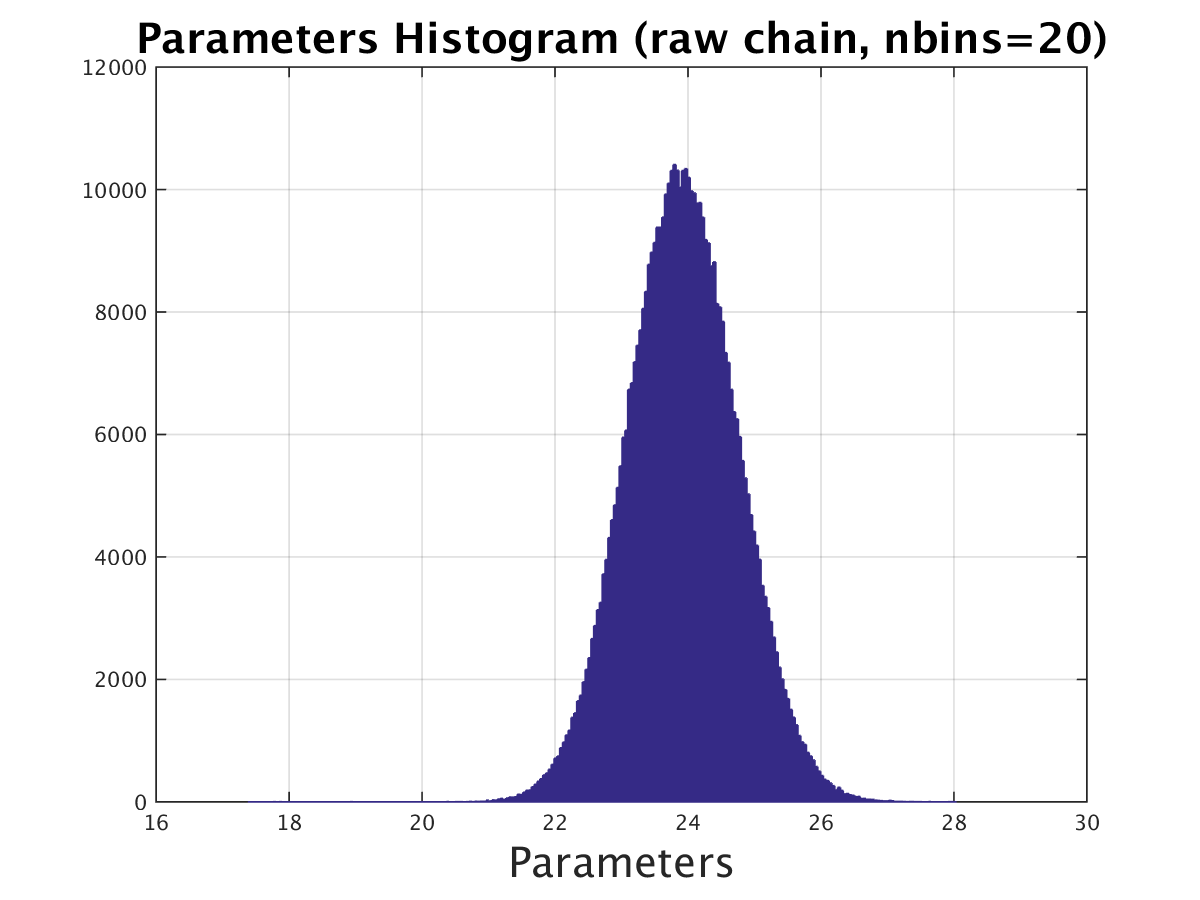
\includegraphics[scale=0.75]{100_results/outputData_100/simple_ip_hist_raw}
   \caption{Histogram}
\end{figure}
%
%
%
\begin{figure}[H]
  
  \centering
   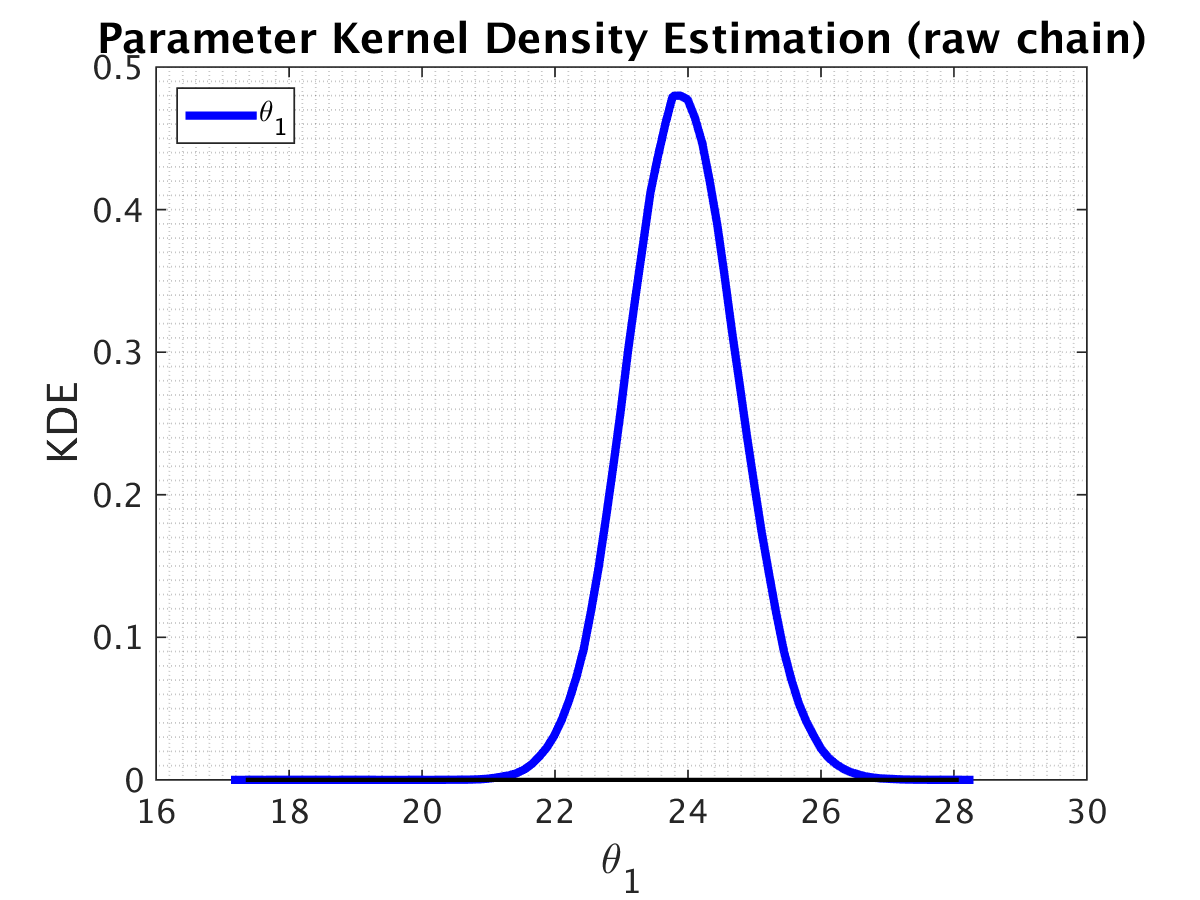
\includegraphics[scale=0.75]{100_results/outputData_100/simple_ip_kde_raw}
   \caption{ KDE }
\end{figure}
%
\clearpage

\begin{figure}[H]
  
  \centering
   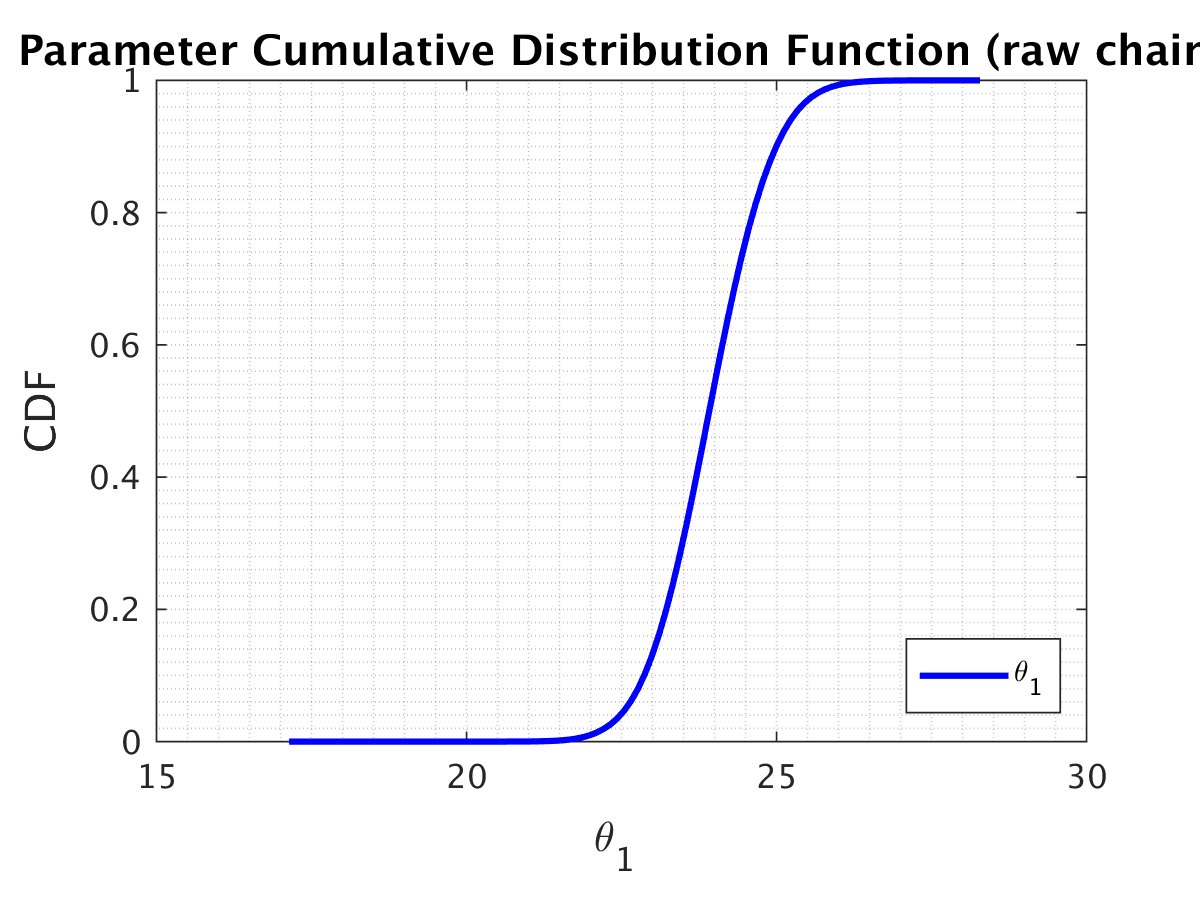
\includegraphics[scale=0.75]{100_results/outputData_100/simple_ip_cdf_raw}
   \caption{CDF function for Parameter }
\end{figure}

\clearpage

\begin{figure}[H]
  
  \centering
   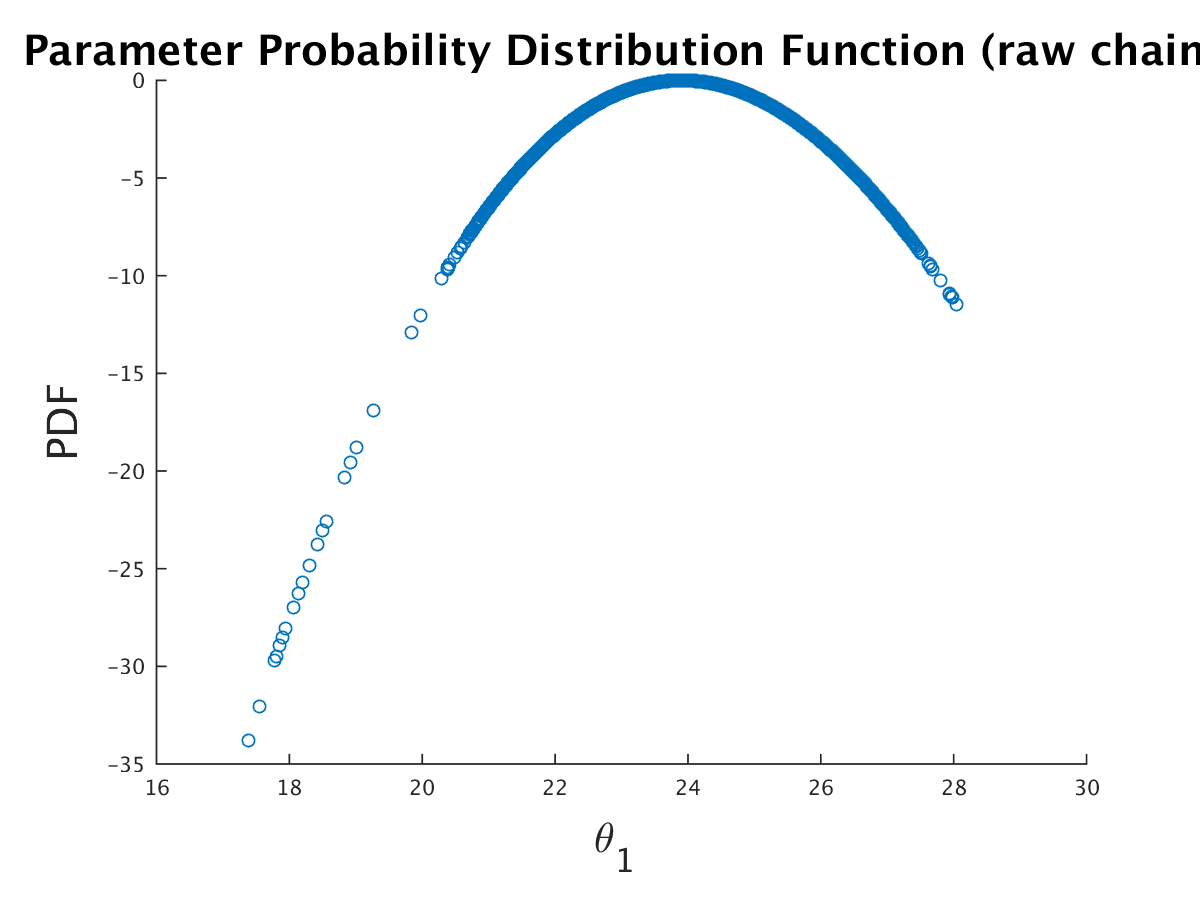
\includegraphics[scale=0.75]{100_results/outputData_100/ip_logLike_unified}
   \caption{CDF function for Parameter }
\end{figure}


\subsubsection{Sample size (Surrogate size) 500 }

In this section we calculated flamespeed values for 500 points in the domain 

\begin{figure}[H]
  
  \centering
   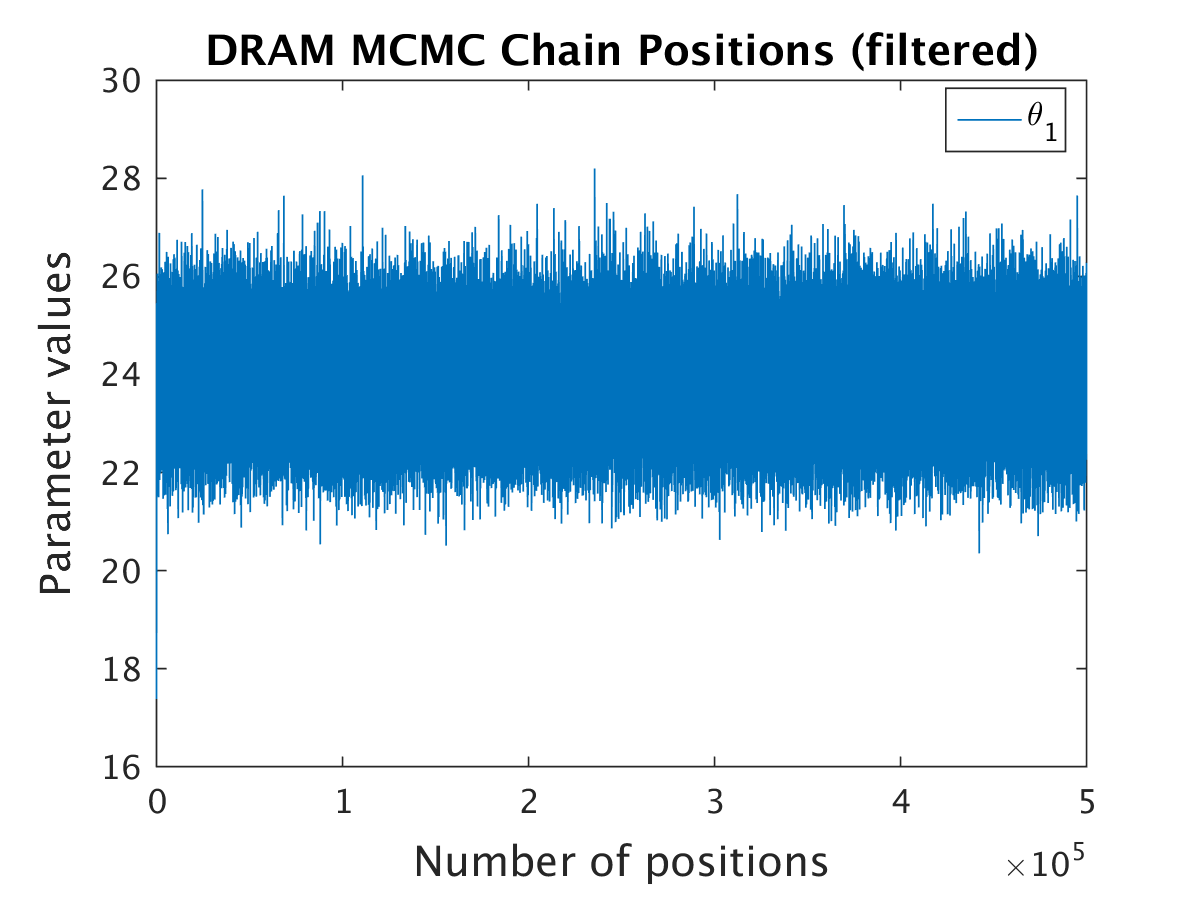
\includegraphics[scale=0.75]{100_results/outputData_500/simple_ip_chain_pos_filt}
   \caption{MCMC chain position }
\end{figure}


\begin{figure}[H]
  
  \centering
   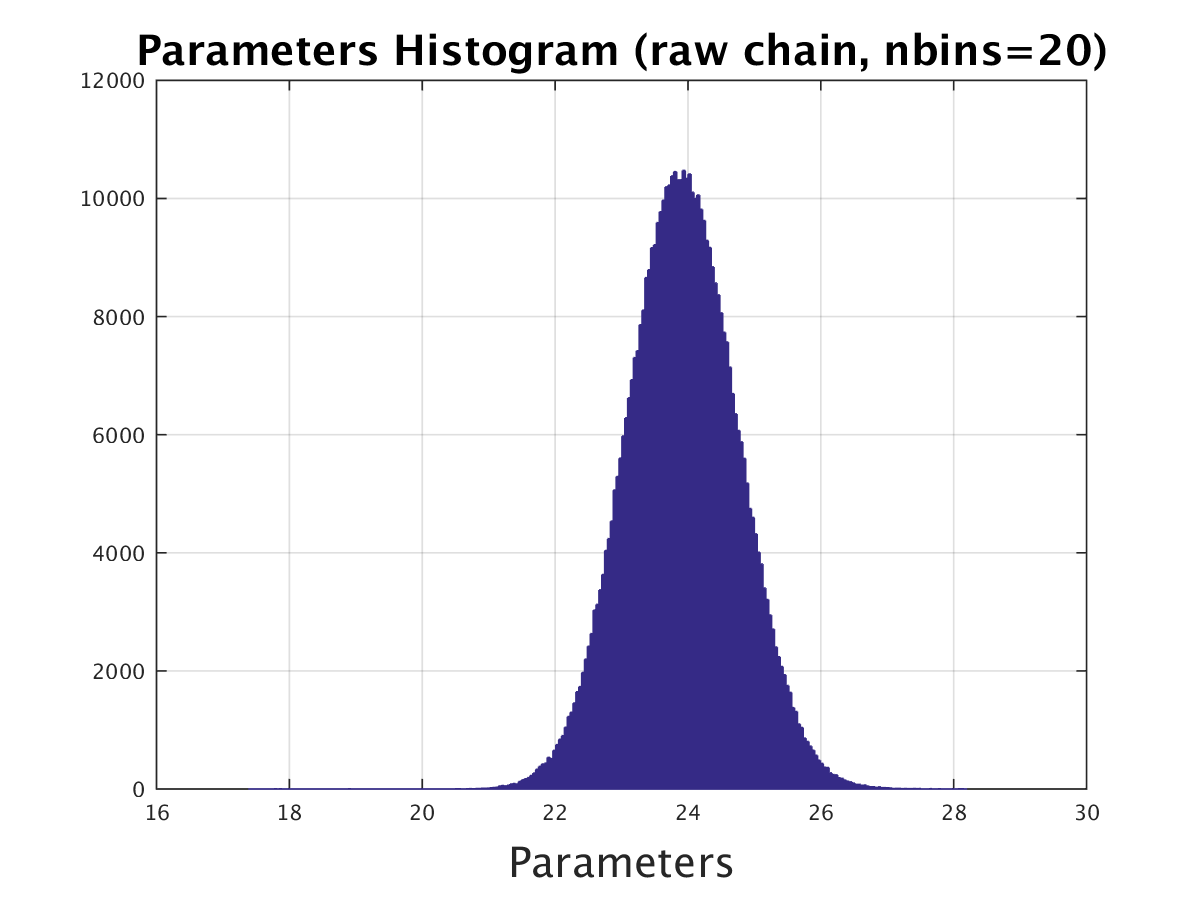
\includegraphics[scale=0.75]{100_results/outputData_500/simple_ip_hist_raw}
   \caption{Histogram}
\end{figure}



\begin{figure}[H]
  
  \centering
   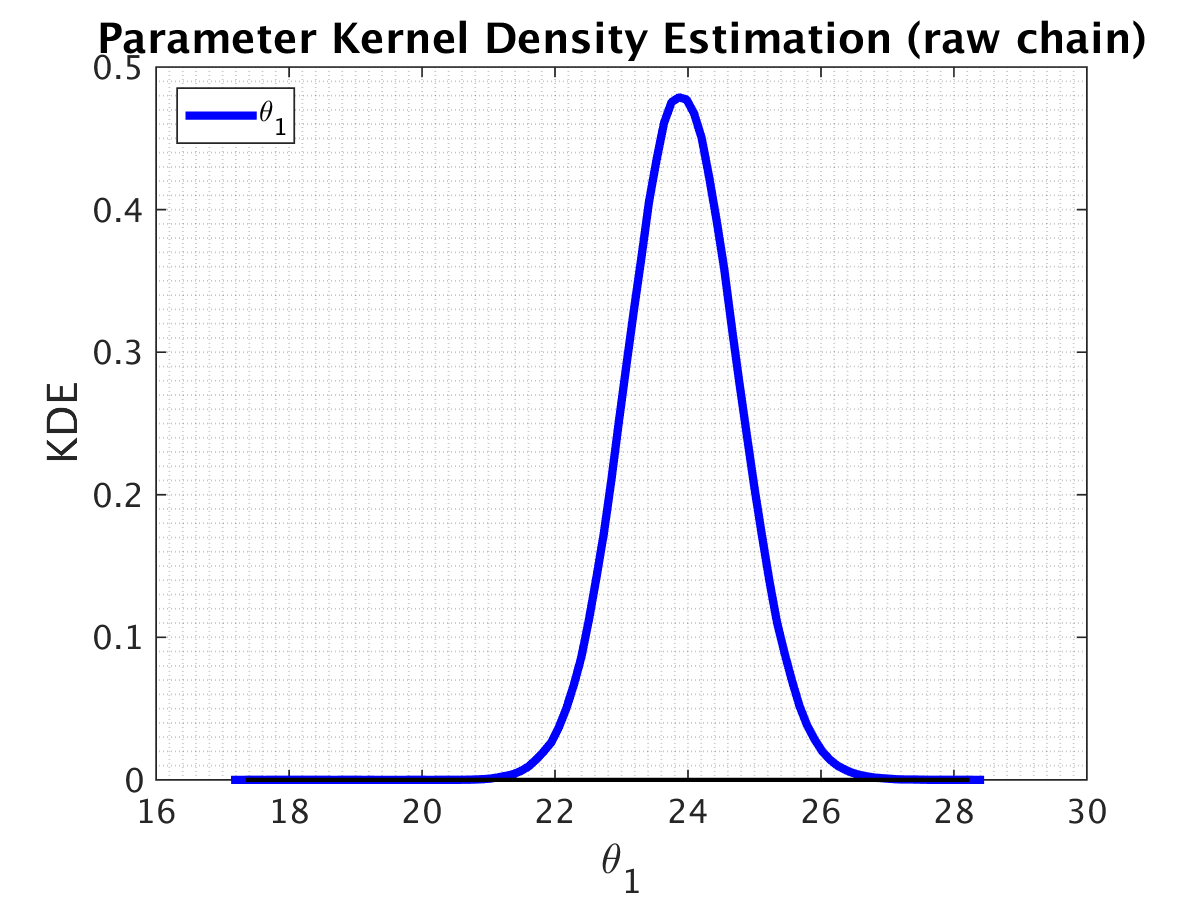
\includegraphics[scale=0.75]{100_results/outputData_500/simple_ip_kde_raw}
   \caption{ KDE }
\end{figure}

\begin{figure}[H]
  
  \centering
   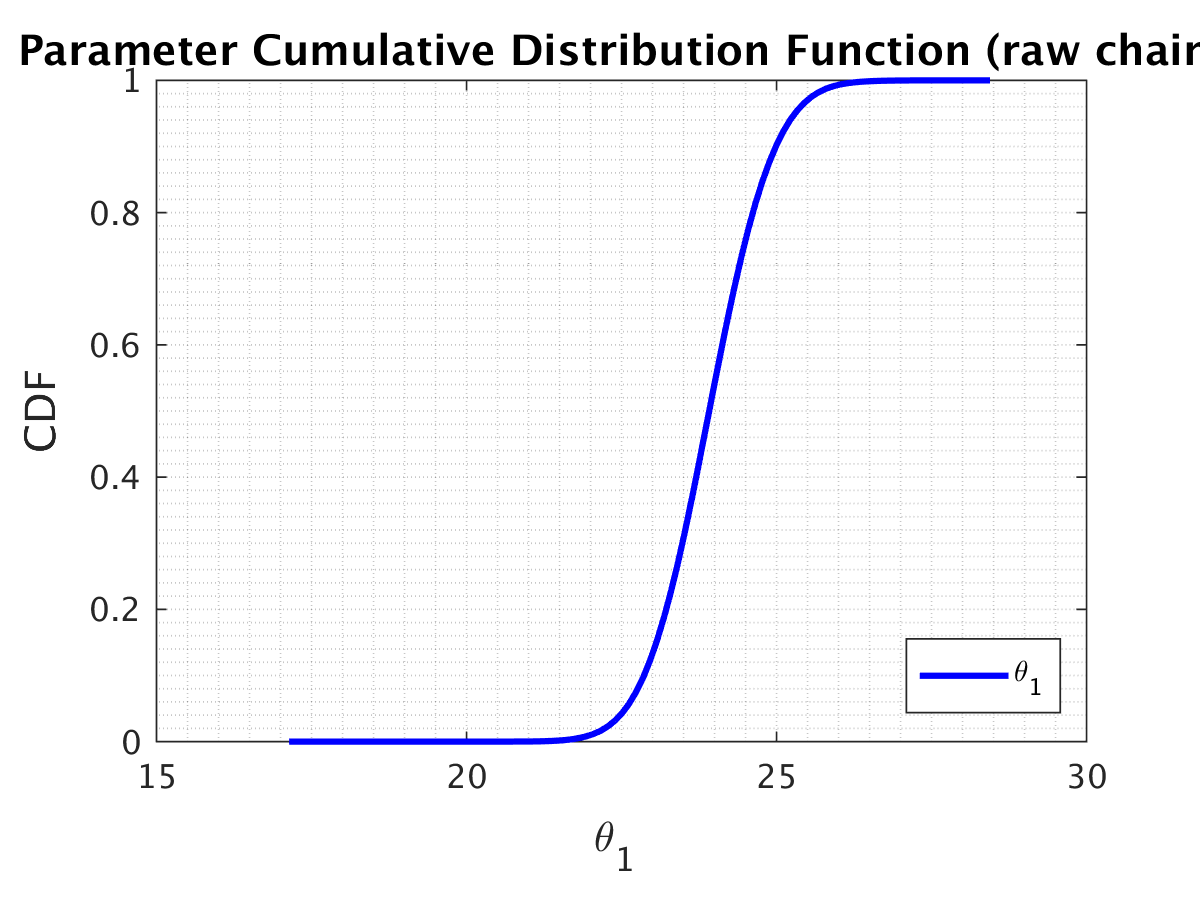
\includegraphics[scale=0.75]{100_results/outputData_500/simple_ip_cdf_raw}
   \caption{CDF function for Parameter }
\end{figure}



\begin{figure}[H]
  
  \centering
   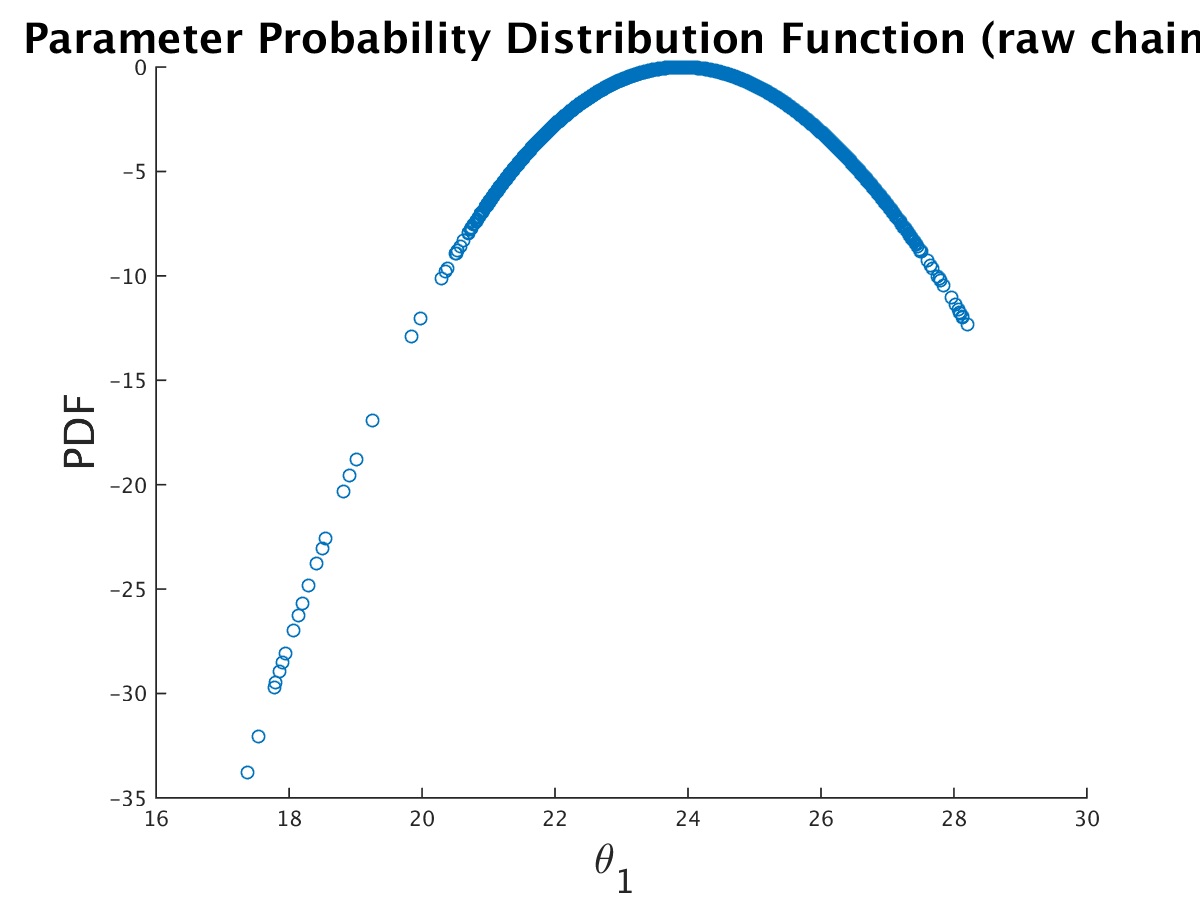
\includegraphics[scale=0.75]{100_results/outputData_500/ip_logLike_unified}
   \caption{PDF function for Parameter }
\end{figure}


\subsubsection{Sample size (Surrogate size) 1000 }

In this section we calculated flamespeed values for 1000 points in the domain 

\begin{figure}[H]
  
  \centering
   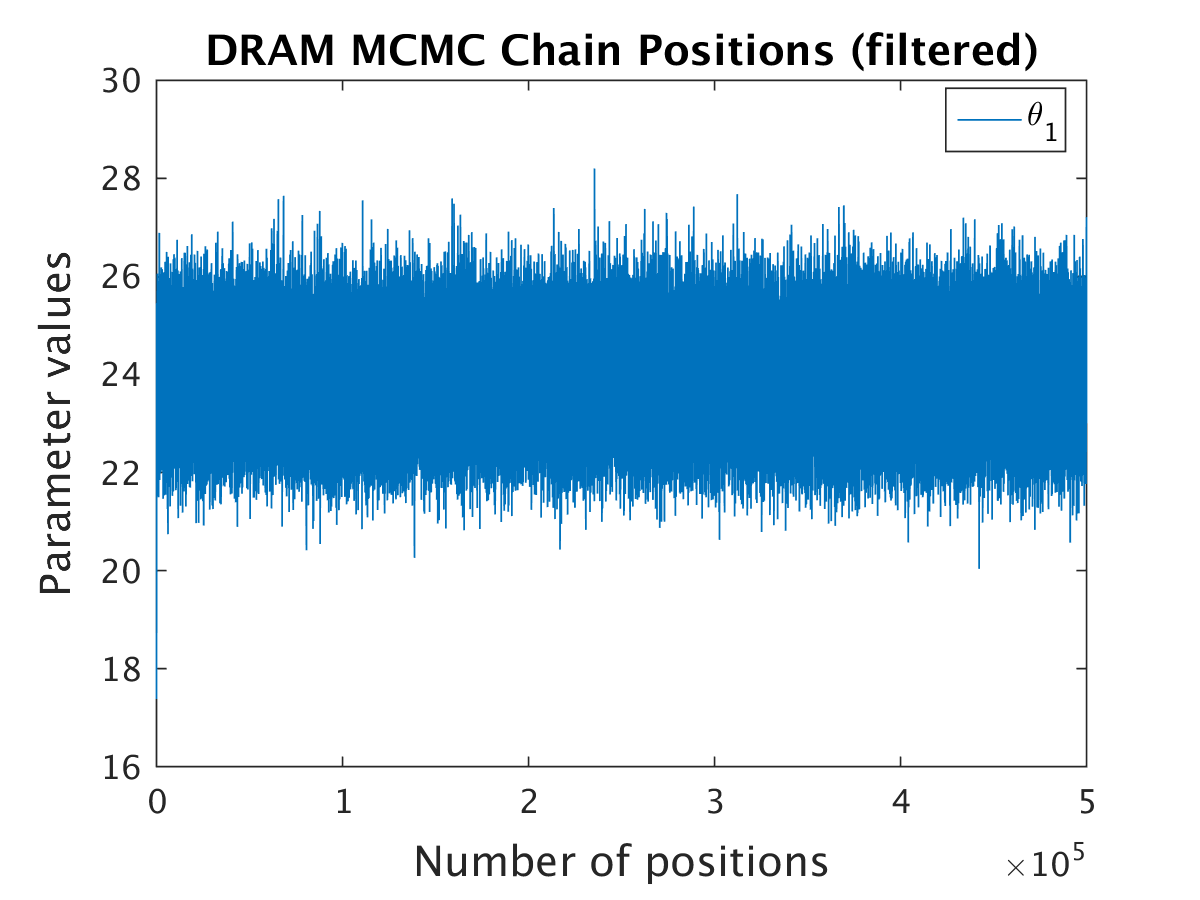
\includegraphics[scale=0.75]{100_results/outputData_1000/simple_ip_chain_pos_filt}
   \caption{MCMC chain position }
\end{figure}


\begin{figure}[H]
  
  \centering
   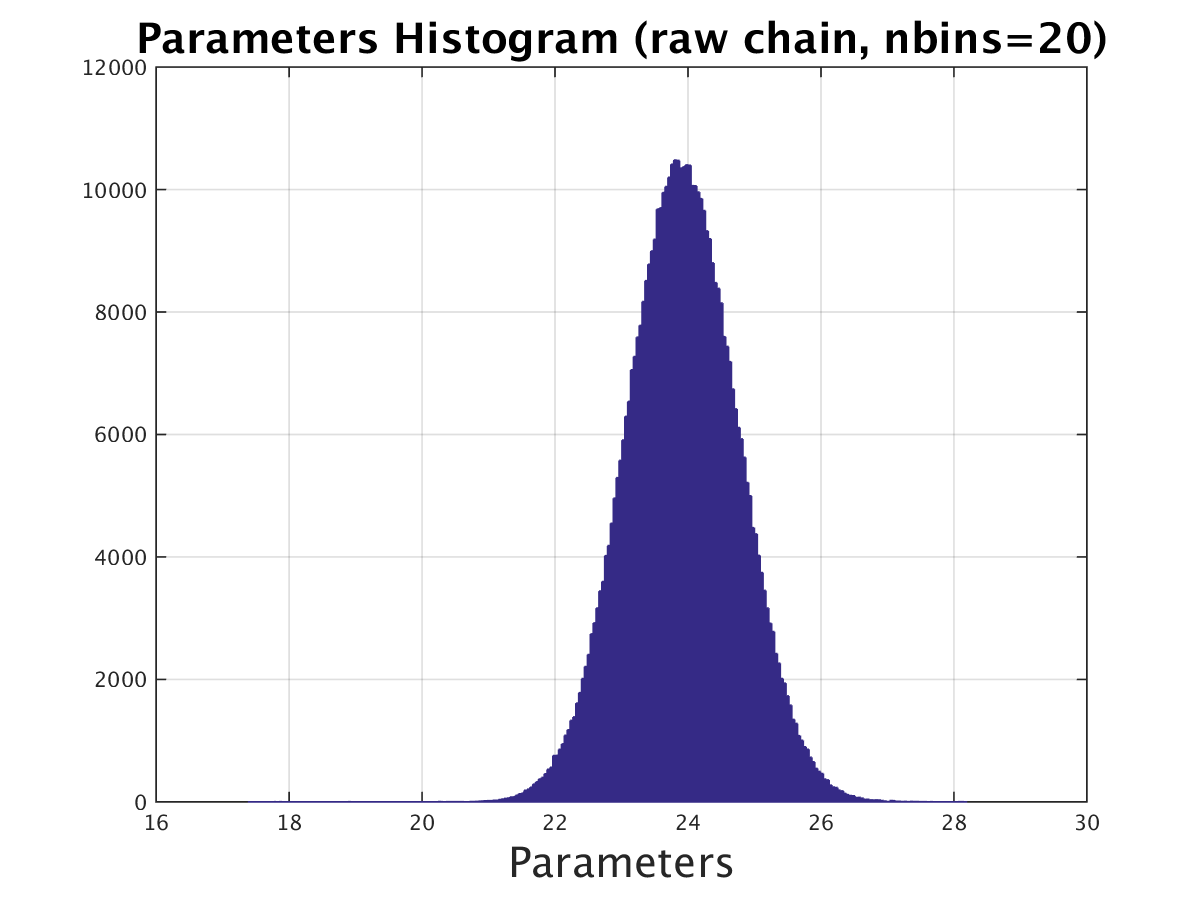
\includegraphics[scale=0.75]{100_results/outputData_1000/simple_ip_hist_raw}
   \caption{Histogram}
\end{figure}



\begin{figure}[H]
  
  \centering
   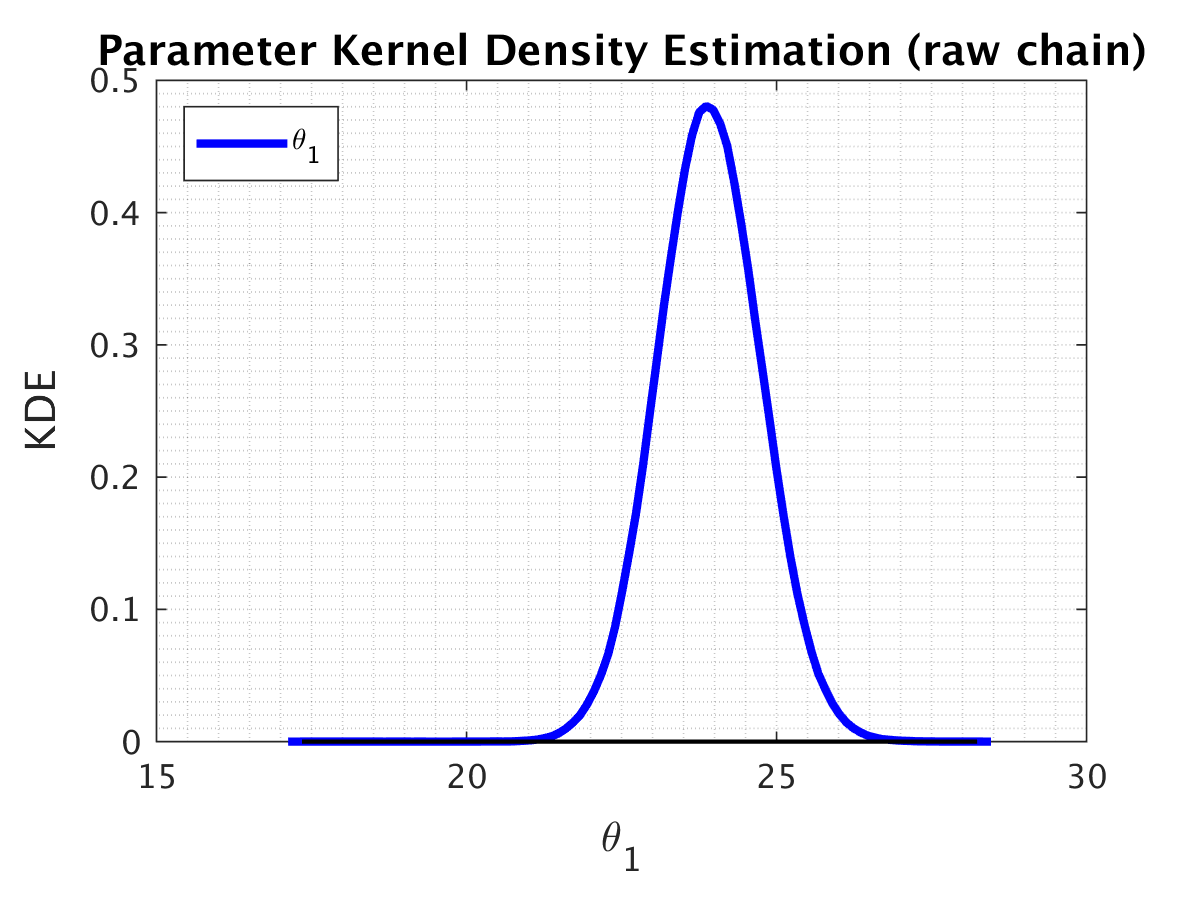
\includegraphics[scale=0.75]{100_results/outputData_1000/simple_ip_kde_raw}
   \caption{ KDE }
\end{figure}

\begin{figure}[H]
  
  \centering
   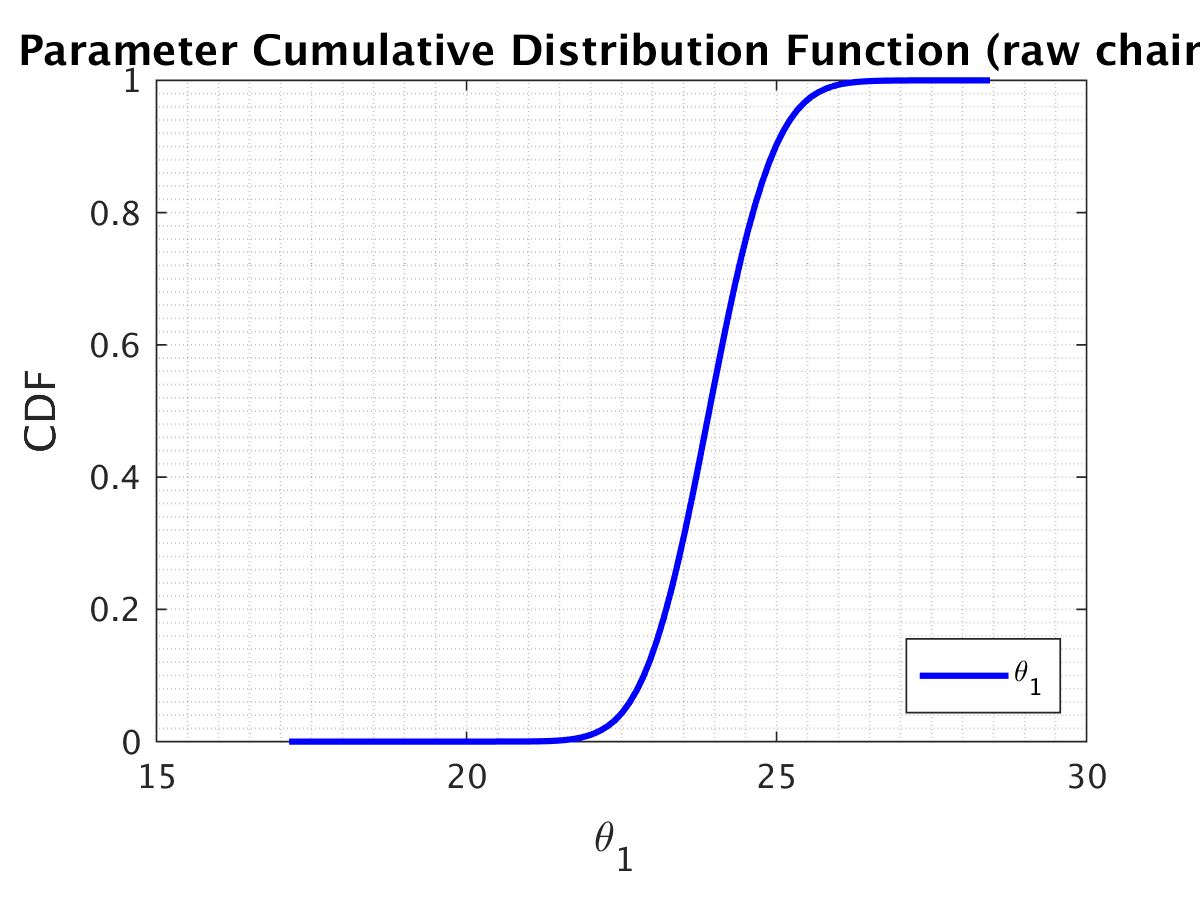
\includegraphics[scale=0.75]{100_results/outputData_1000/simple_ip_cdf_raw}
   \caption{CDF function for Parameter }
\end{figure}



\begin{figure}[H]
  
  \centering
   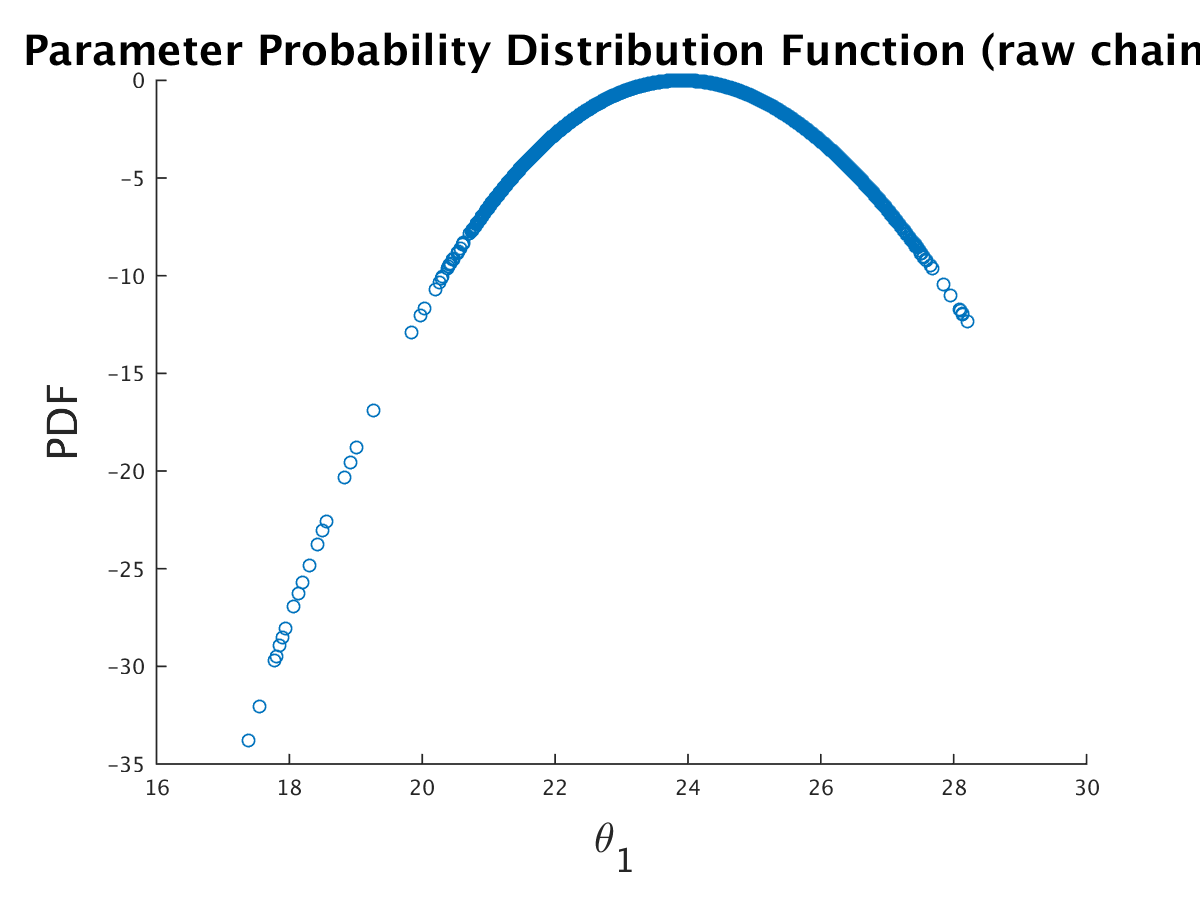
\includegraphics[scale=0.75]{100_results/outputData_1000/ip_logLike_unified}
   \caption{PDF function for Parameter }
\end{figure}


\subsubsection{Different chain sizes }

In this section we calculated flamespeed values for 100 different points in the domain and the remaining values are linear combination of these 100. we change the size of raw chain (mcmc chain size). 

\subsubsection{Chain size 100000 }

In this section we have chain size of 100000 points. 

\begin{figure}[H]
  
  \centering
   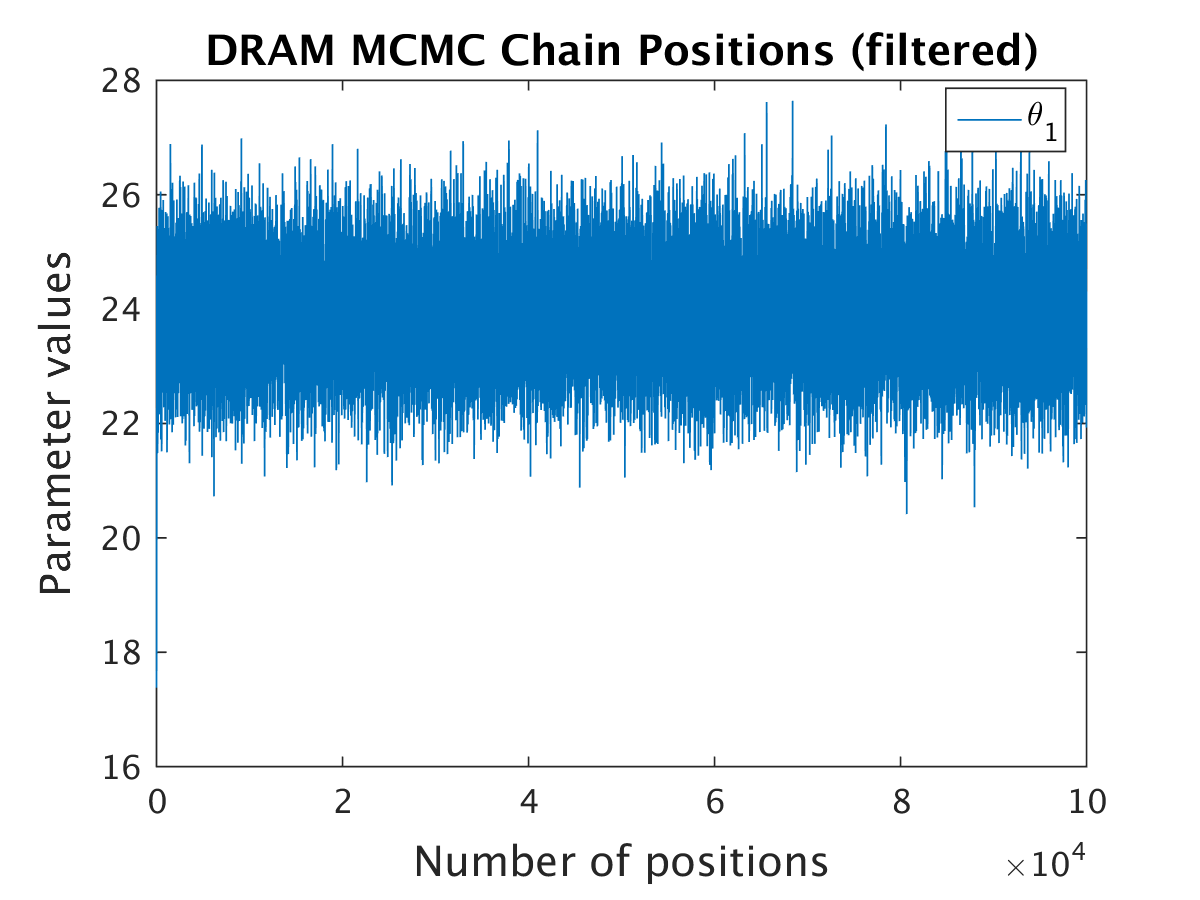
\includegraphics[scale=0.75]{100_results/outputData_100000/simple_ip_chain_pos_filt}
   \caption{MCMC chain position }
\end{figure}


\begin{figure}[H]
  
  \centering
   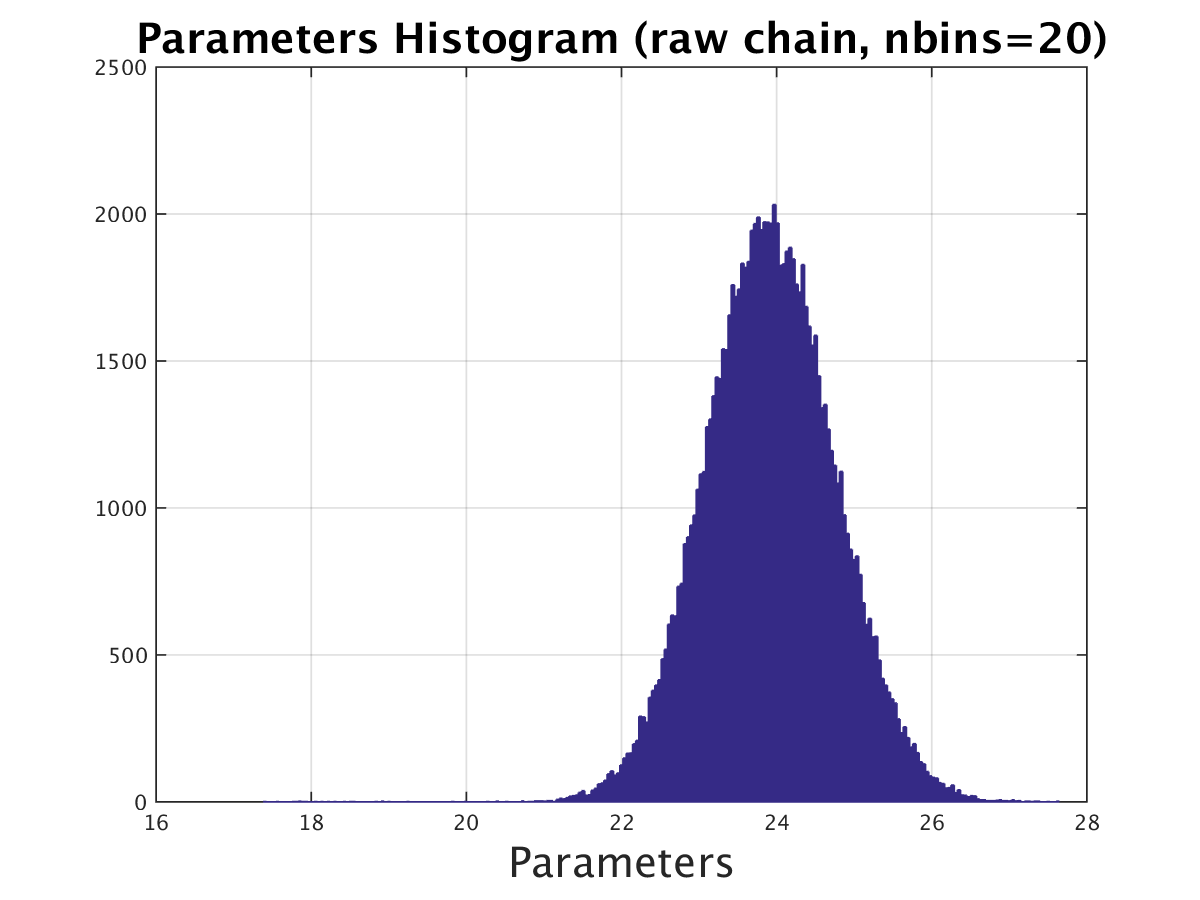
\includegraphics[scale=0.75]{100_results/outputData_100000/simple_ip_hist_raw}
   \caption{Histogram}
\end{figure}



\begin{figure}[H]
  
  \centering
   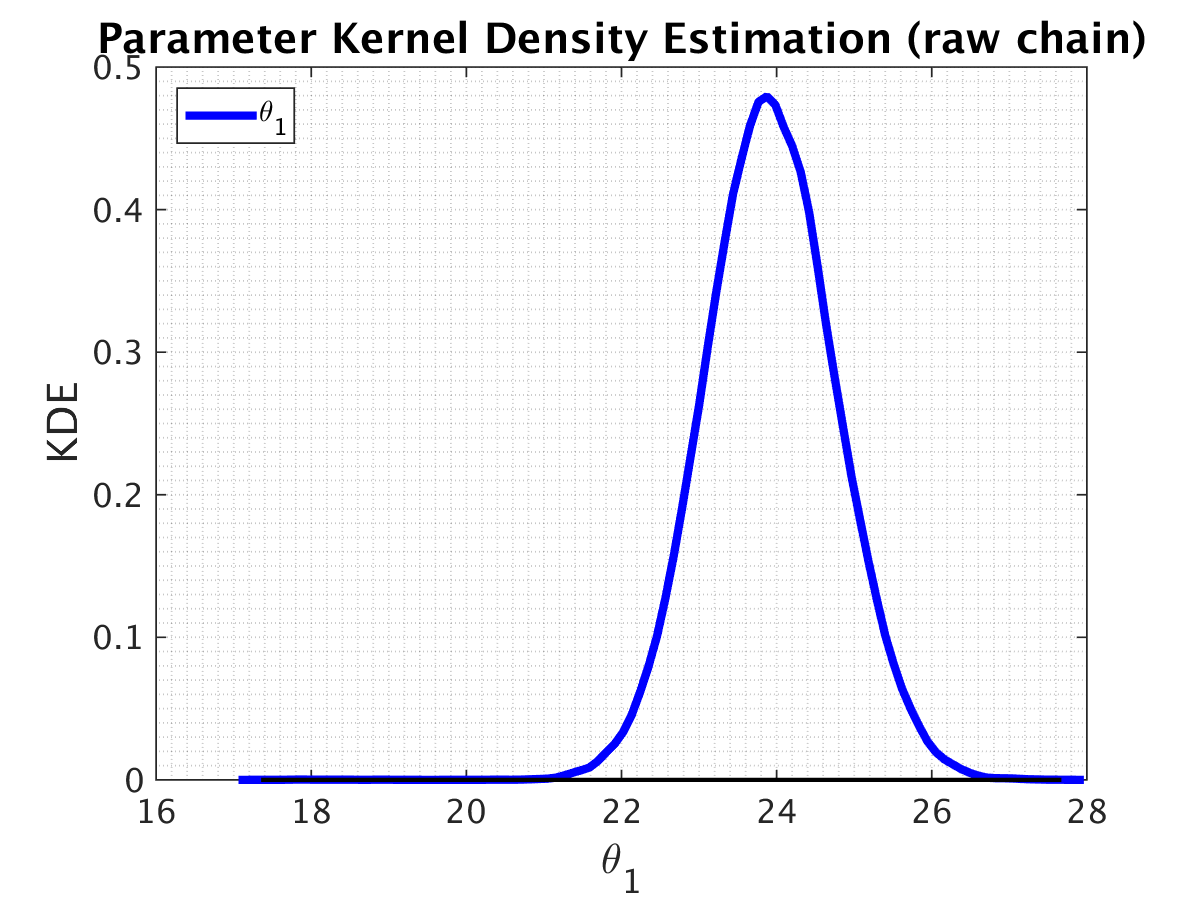
\includegraphics[scale=0.75]{100_results/outputData_100000/simple_ip_kde_raw}
   \caption{ KDE }
\end{figure}

\begin{figure}[H]
  
  \centering
   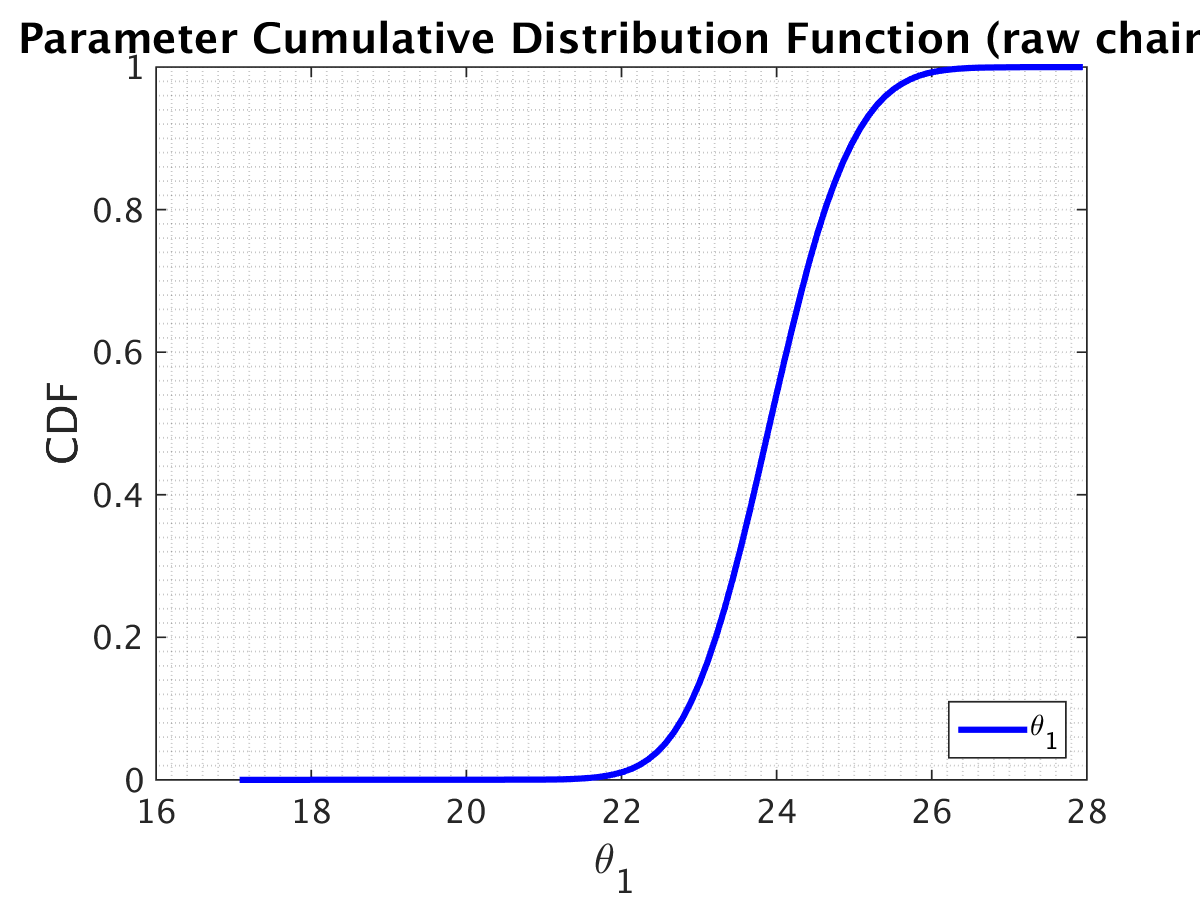
\includegraphics[scale=0.75]{100_results/outputData_100000/simple_ip_cdf_raw}
   \caption{CDF function for Parameter }
\end{figure}



\begin{figure}[H]
  
  \centering
   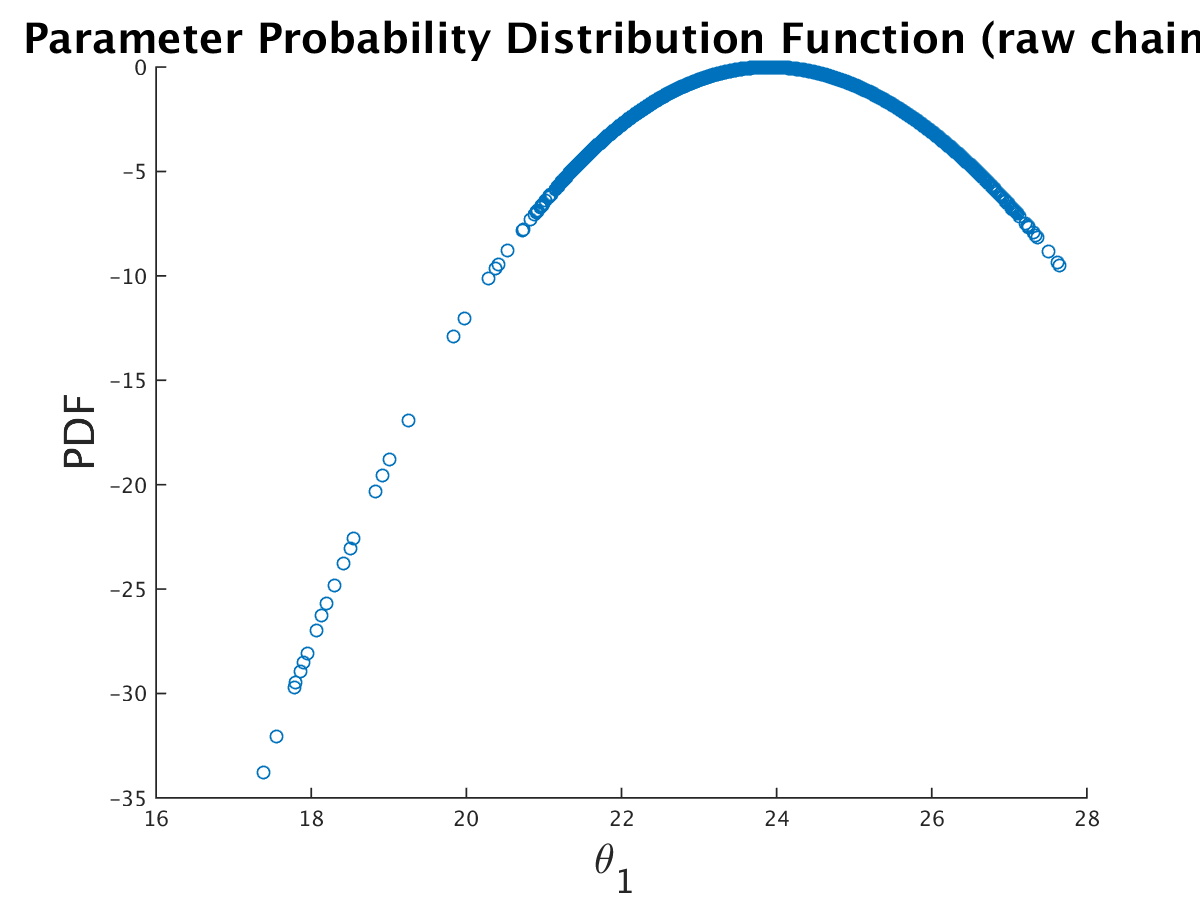
\includegraphics[scale=0.75]{100_results/outputData_100000/ip_logLike_unified}
   \caption{PDF function for Parameter }
\end{figure}


\subsubsection{Chain size 300000 }


In this section we have chain size of 300000 points. 

\begin{figure}[H]
  
  \centering
   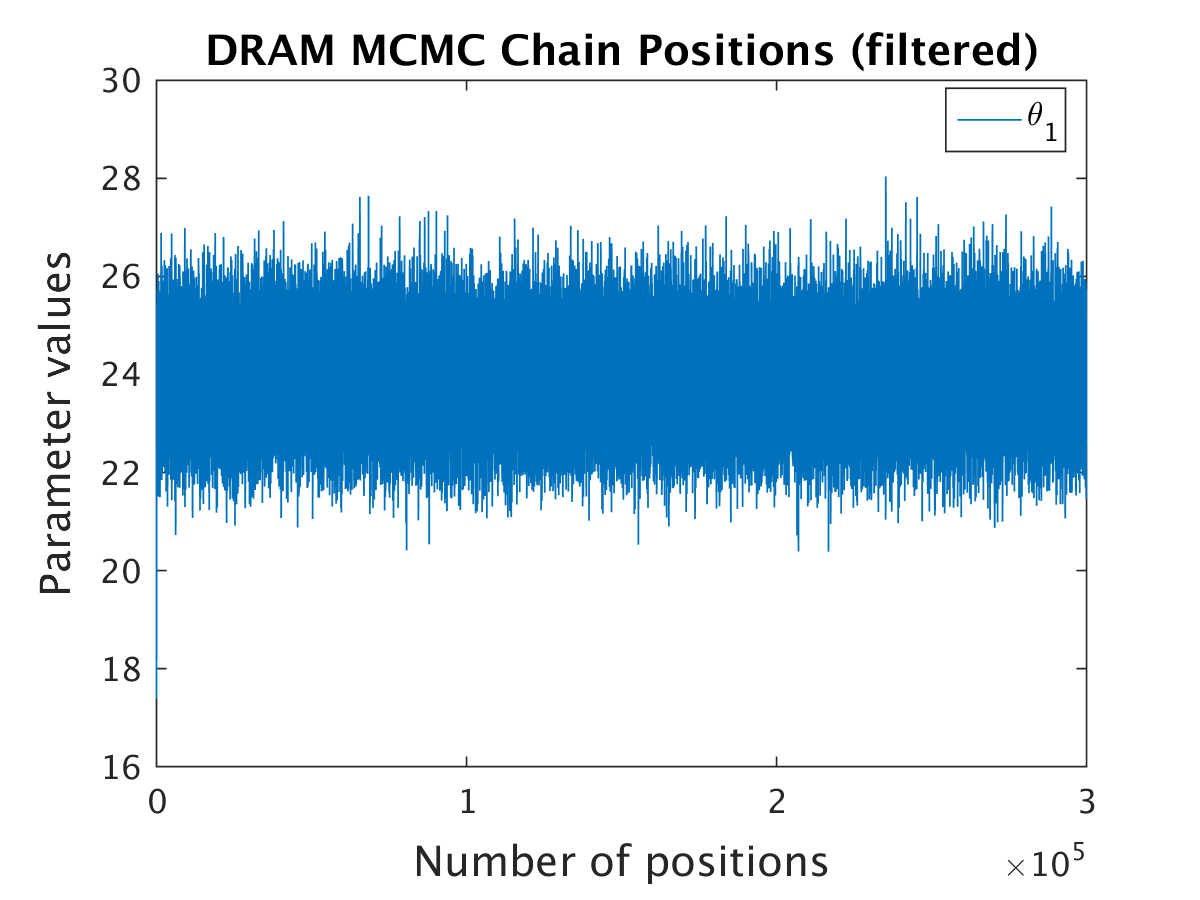
\includegraphics[scale=0.75]{100_results/outputData_300000/simple_ip_chain_pos_filt}
   \caption{MCMC chain position }
\end{figure}


\begin{figure}[H]
  
  \centering
   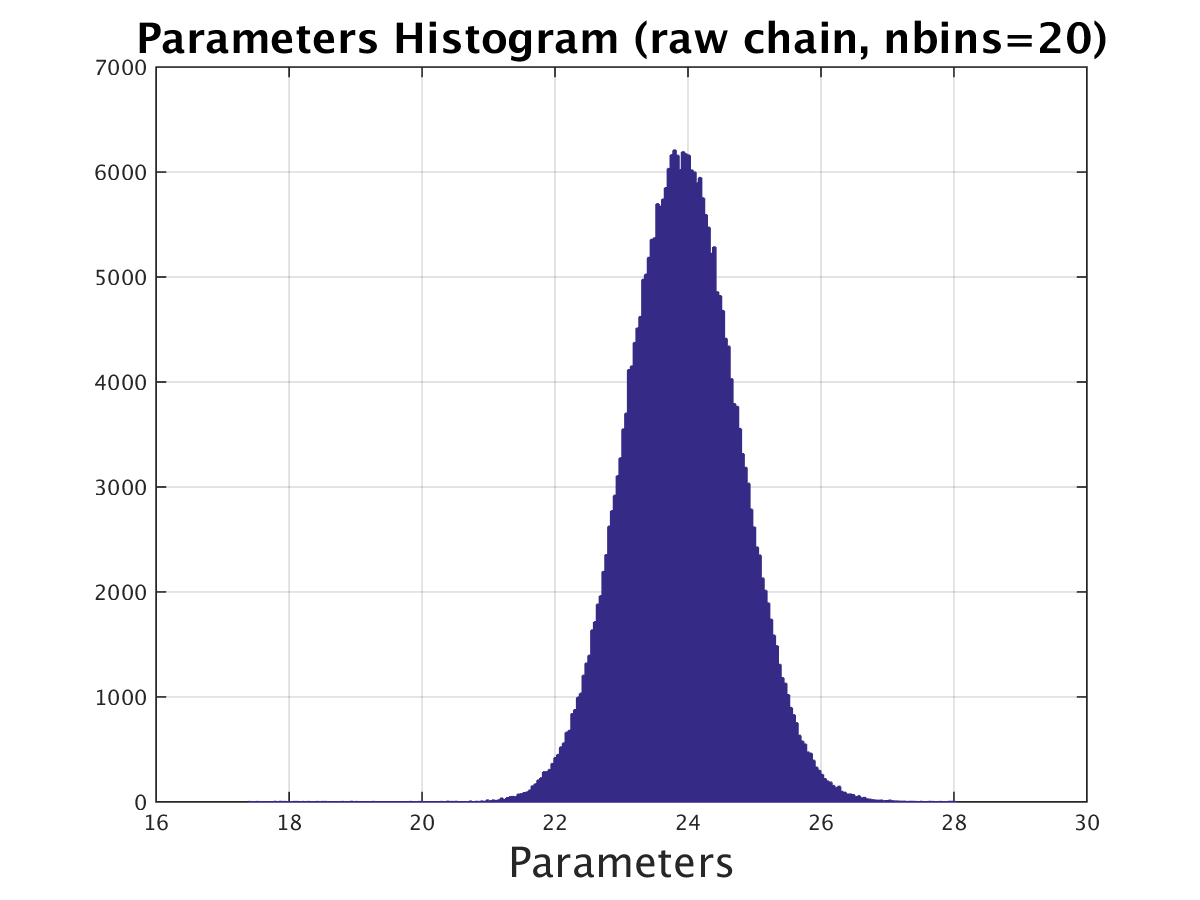
\includegraphics[scale=0.75]{100_results/outputData_300000/simple_ip_hist_raw}
   \caption{Histogram}
\end{figure}

\clearpage

\begin{figure}[H]
  
  \centering
   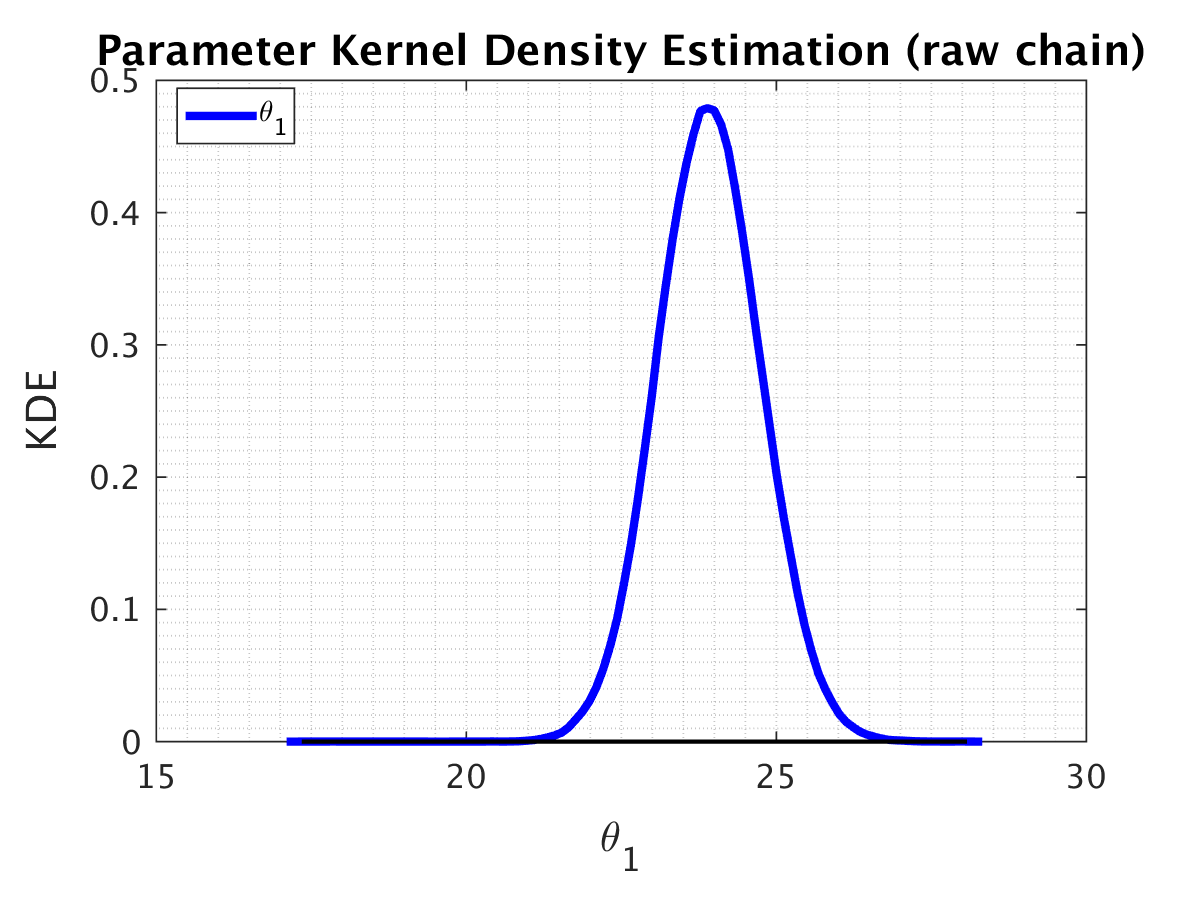
\includegraphics[scale=0.75]{100_results/outputData_300000/simple_ip_kde_raw}
   \caption{ KDE }
\end{figure}

\begin{figure}[H]
  
  \centering
   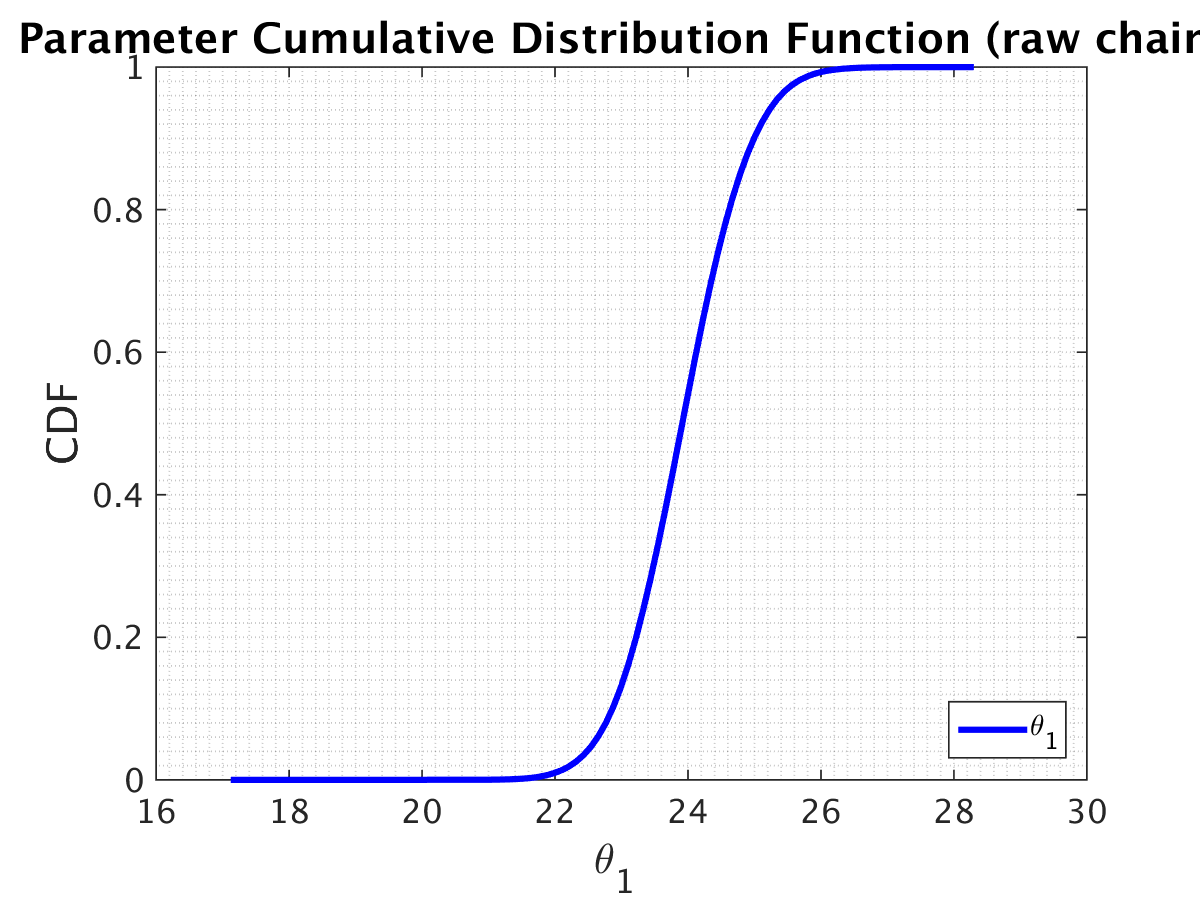
\includegraphics[scale=0.75]{100_results/outputData_300000/simple_ip_cdf_raw}
   \caption{CDF function for Parameter }
\end{figure}



\begin{figure}[H]
  
  \centering
   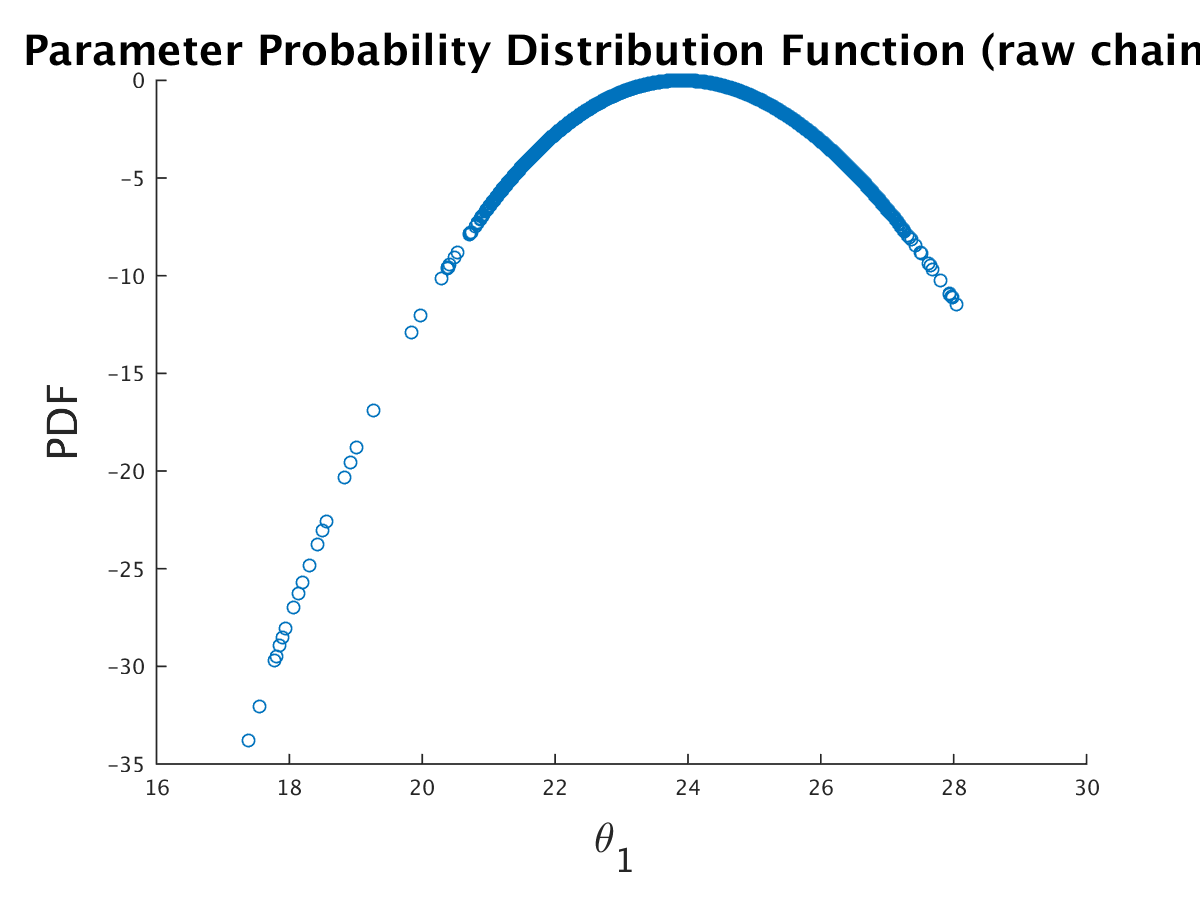
\includegraphics[scale=0.75]{100_results/outputData_300000/ip_logLike_unified}
   \caption{PDF function for Parameter }
\end{figure}


%
\subsubsection{Chain size 700000 }


In this section we have chain size of 700000 points. 

\begin{figure}[H]
  
  \centering
   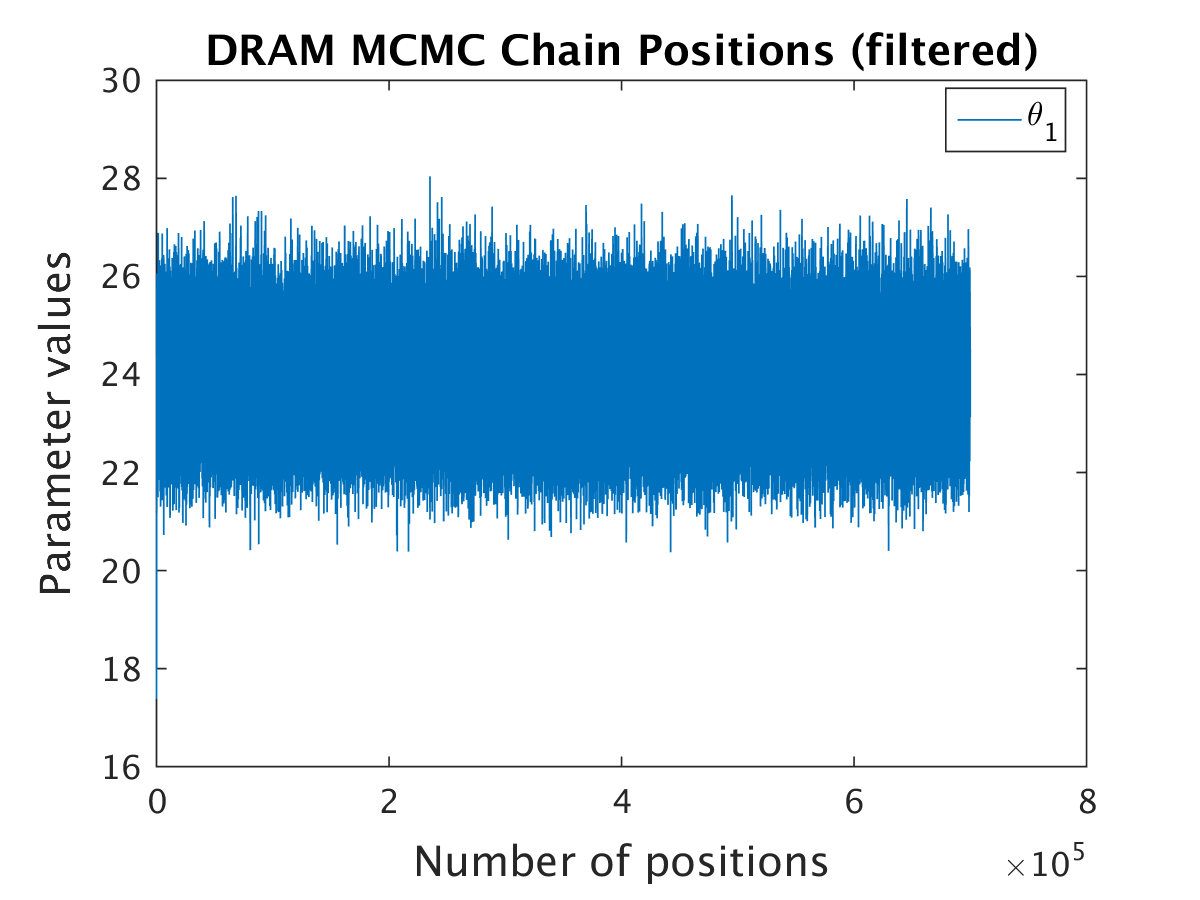
\includegraphics[scale=0.75]{100_results/outputData_700000/simple_ip_chain_pos_filt}
   \caption{MCMC chain position }
\end{figure}


\begin{figure}[H]
  
  \centering
   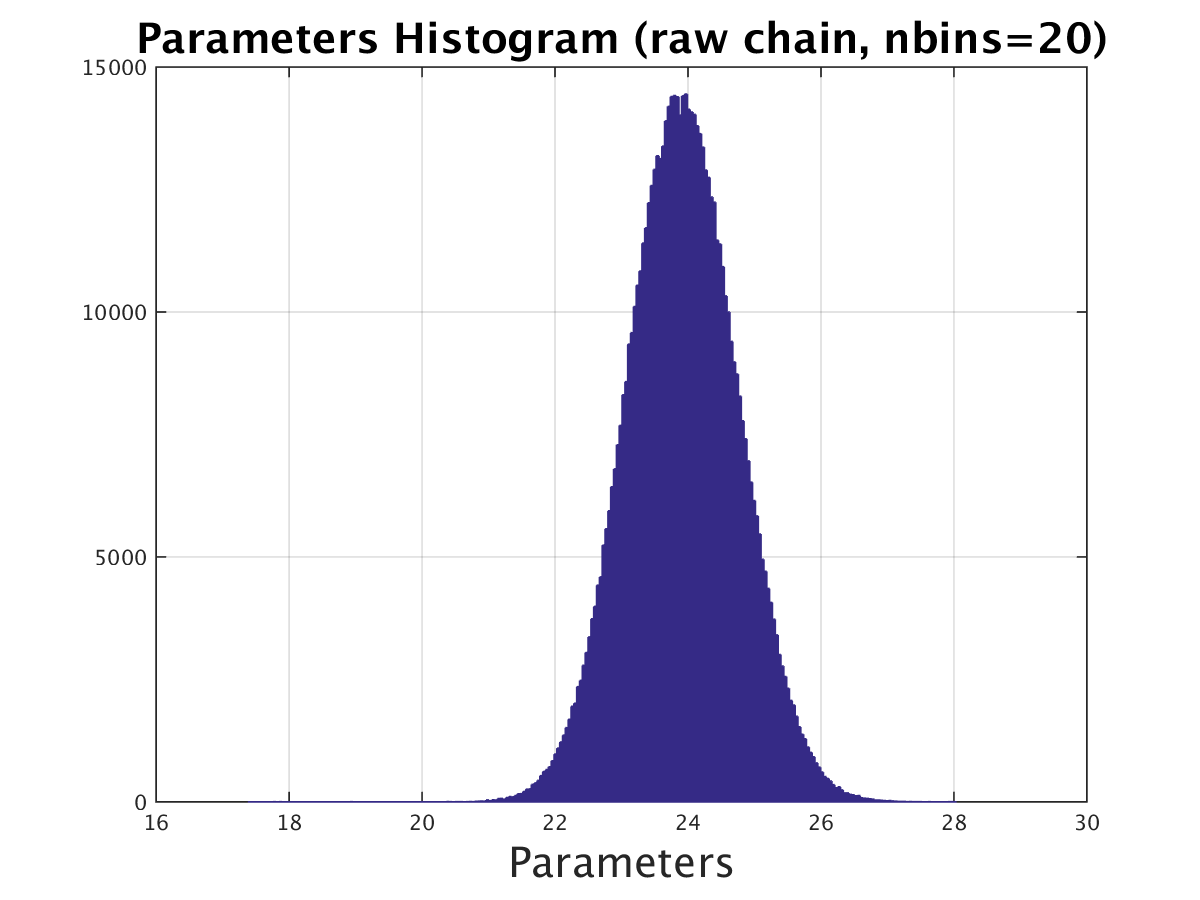
\includegraphics[scale=0.75]{100_results/outputData_700000/simple_ip_hist_raw}
   \caption{Histogram}
\end{figure}



\begin{figure}[H]
  
  \centering
   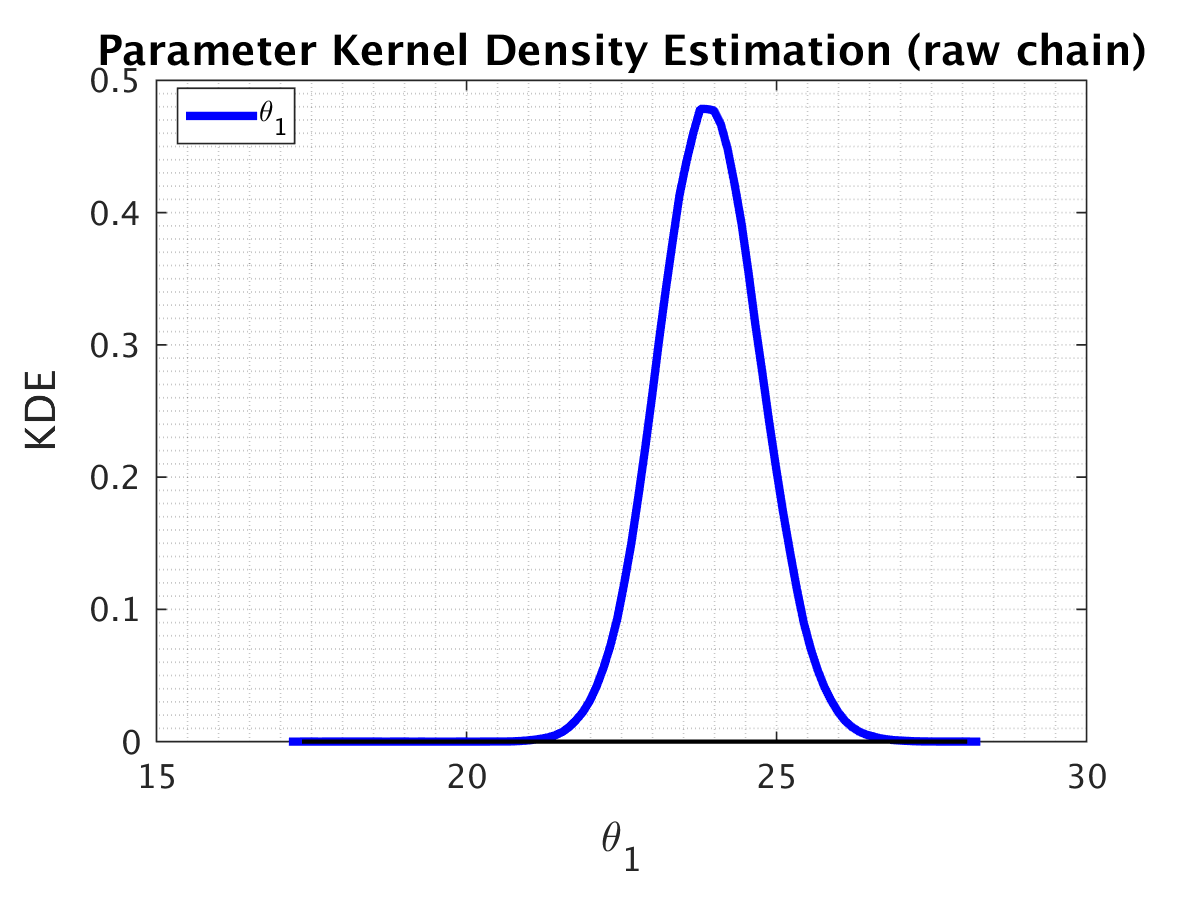
\includegraphics[scale=0.75]{100_results/outputData_700000/simple_ip_kde_raw}
   \caption{ KDE }
\end{figure}

\begin{figure}[H]
  
  \centering
   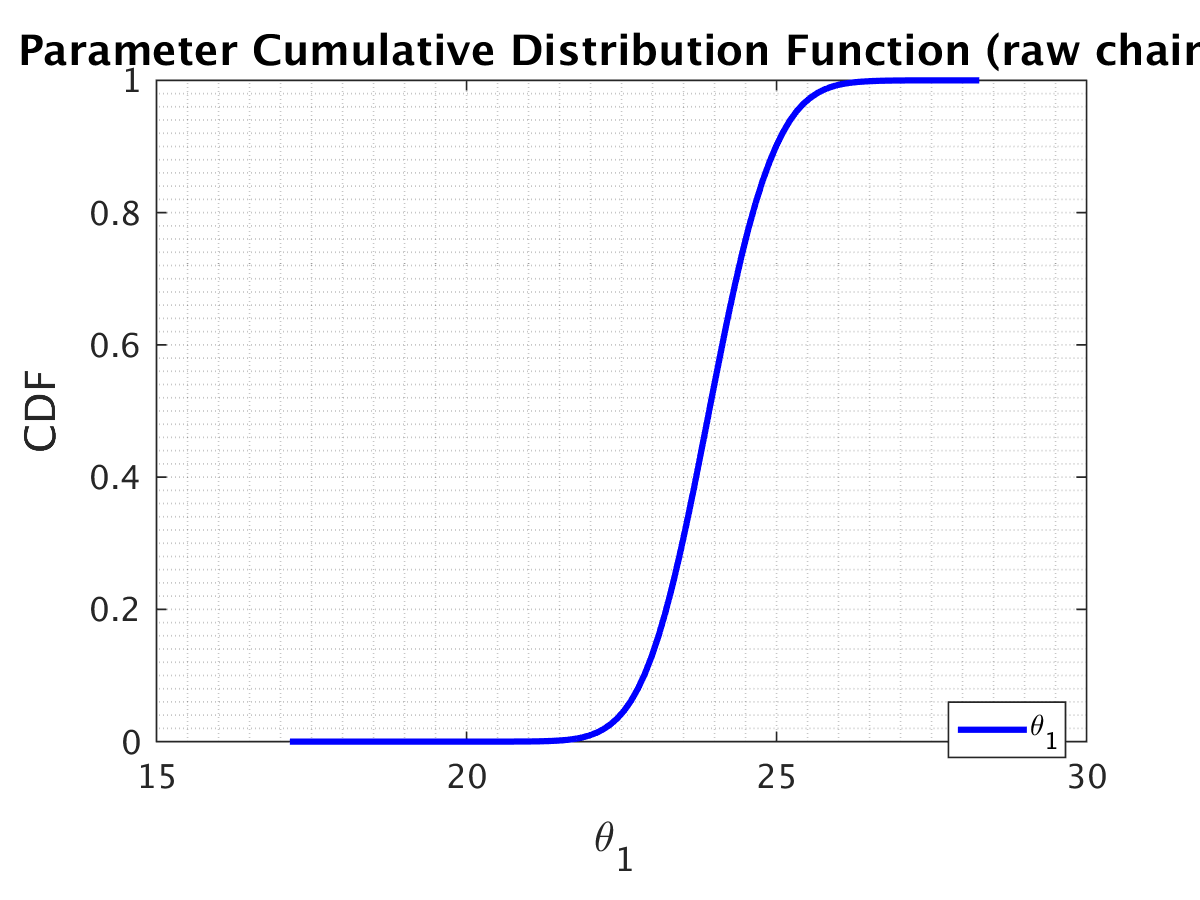
\includegraphics[scale=0.75]{100_results/outputData_700000/simple_ip_cdf_raw}
   \caption{CDF function for Parameter }
\end{figure}



\begin{figure}[H]
  
  \centering
   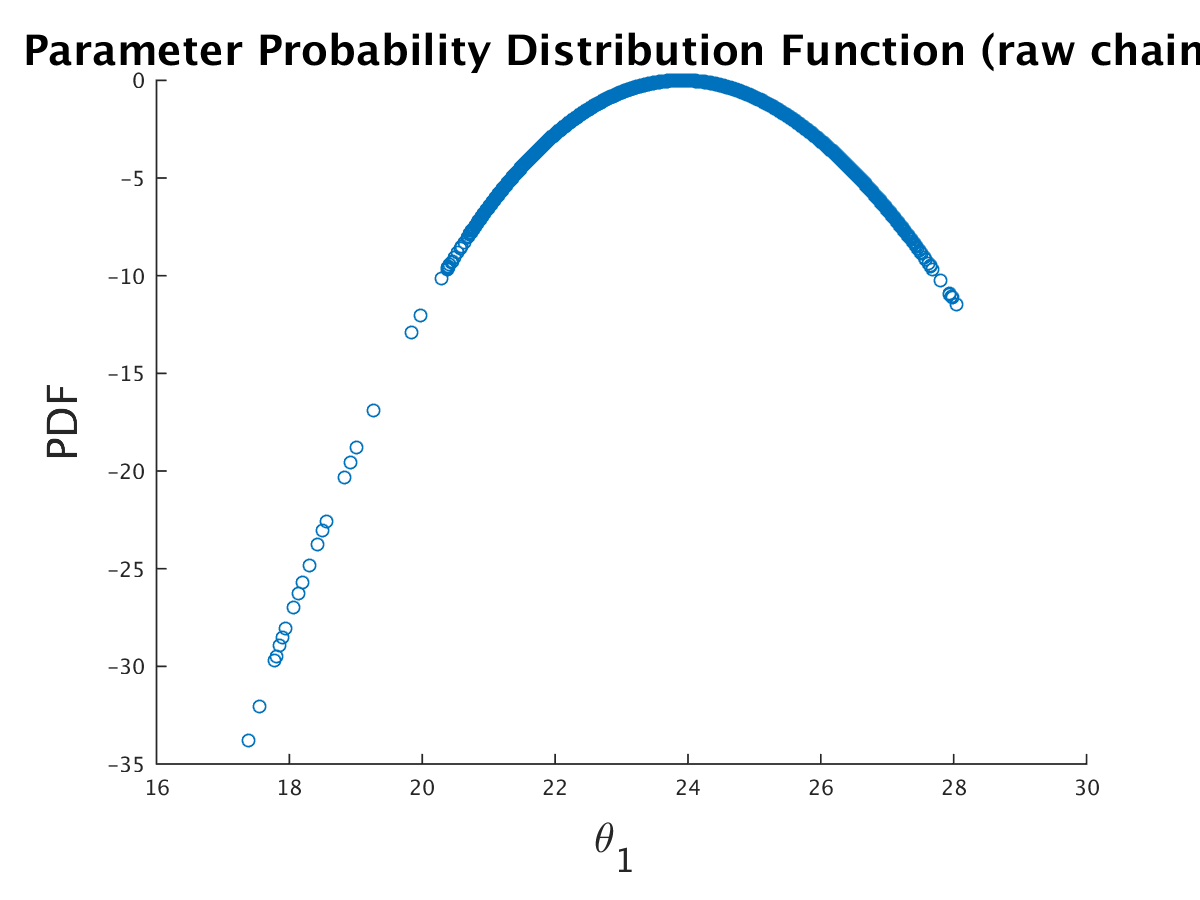
\includegraphics[scale=0.75]{100_results/outputData_700000/ip_logLike_unified}
   \caption{PDF function for Parameter }
\end{figure}



\subsubsection{Chain size 900000 }

In this section we have chain size of 900000 points. 

\begin{figure}[H]
  
  \centering
   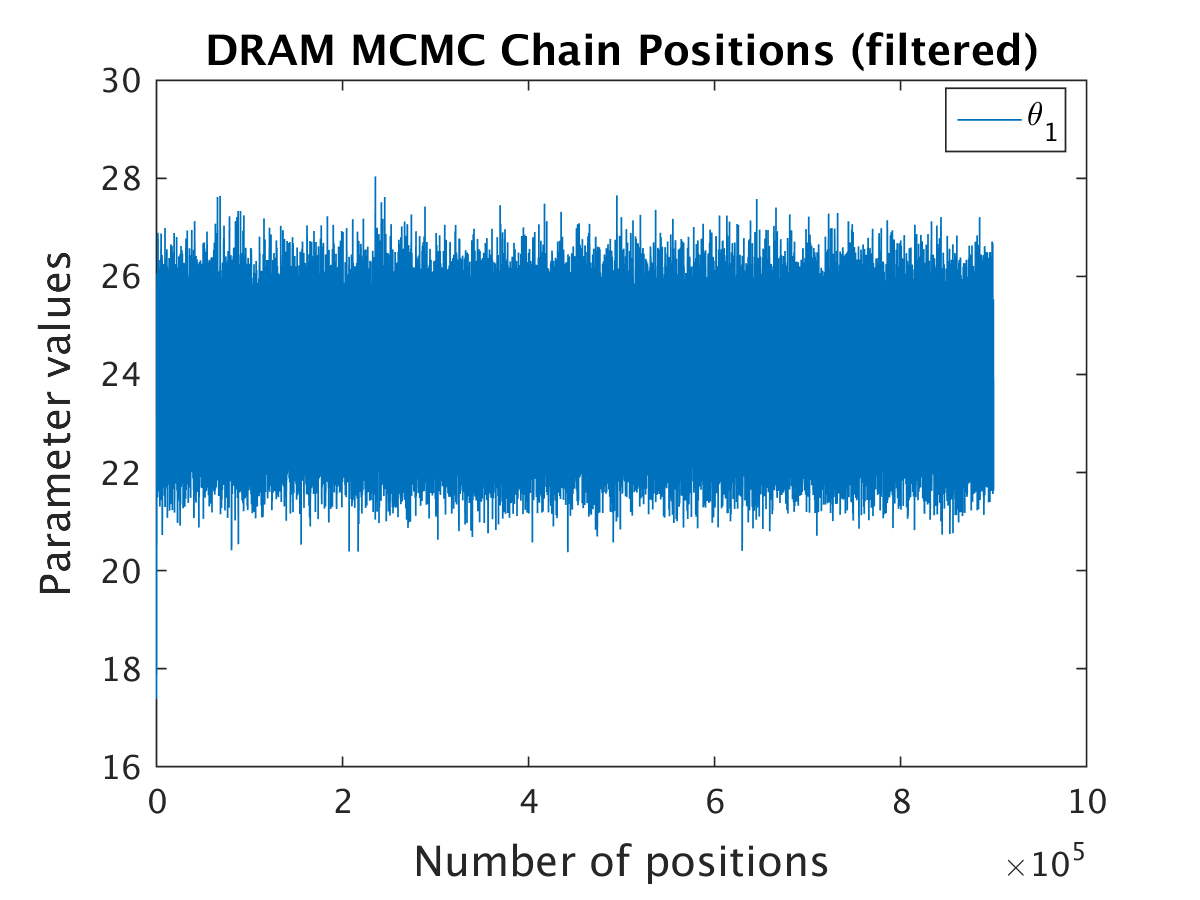
\includegraphics[scale=0.75]{100_results/outputData_900000/simple_ip_chain_pos_filt}
   \caption{MCMC chain position }
\end{figure}


\begin{figure}[H]
  
  \centering
   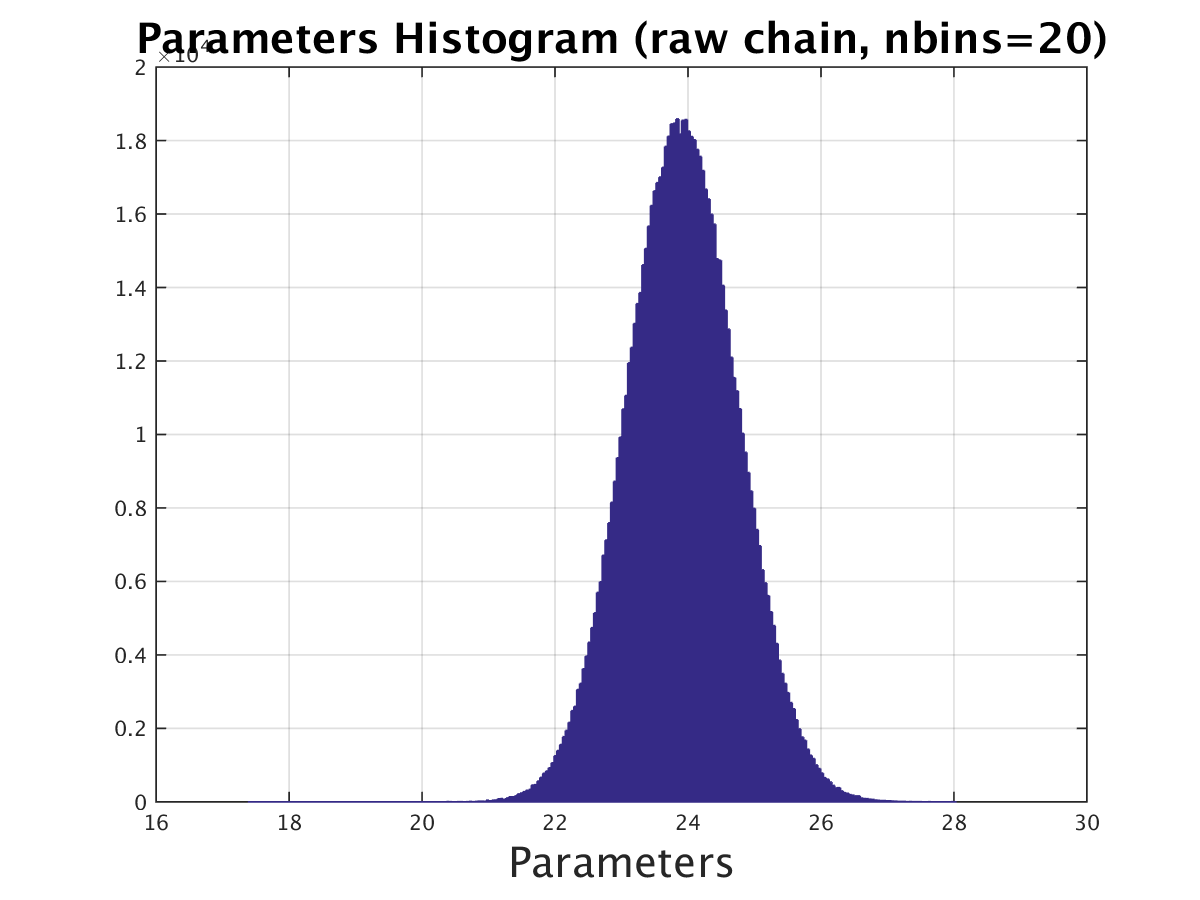
\includegraphics[scale=0.75]{100_results/outputData_900000/simple_ip_hist_raw}
   \caption{Histogram}
\end{figure}



\begin{figure}[H]
  
  \centering
   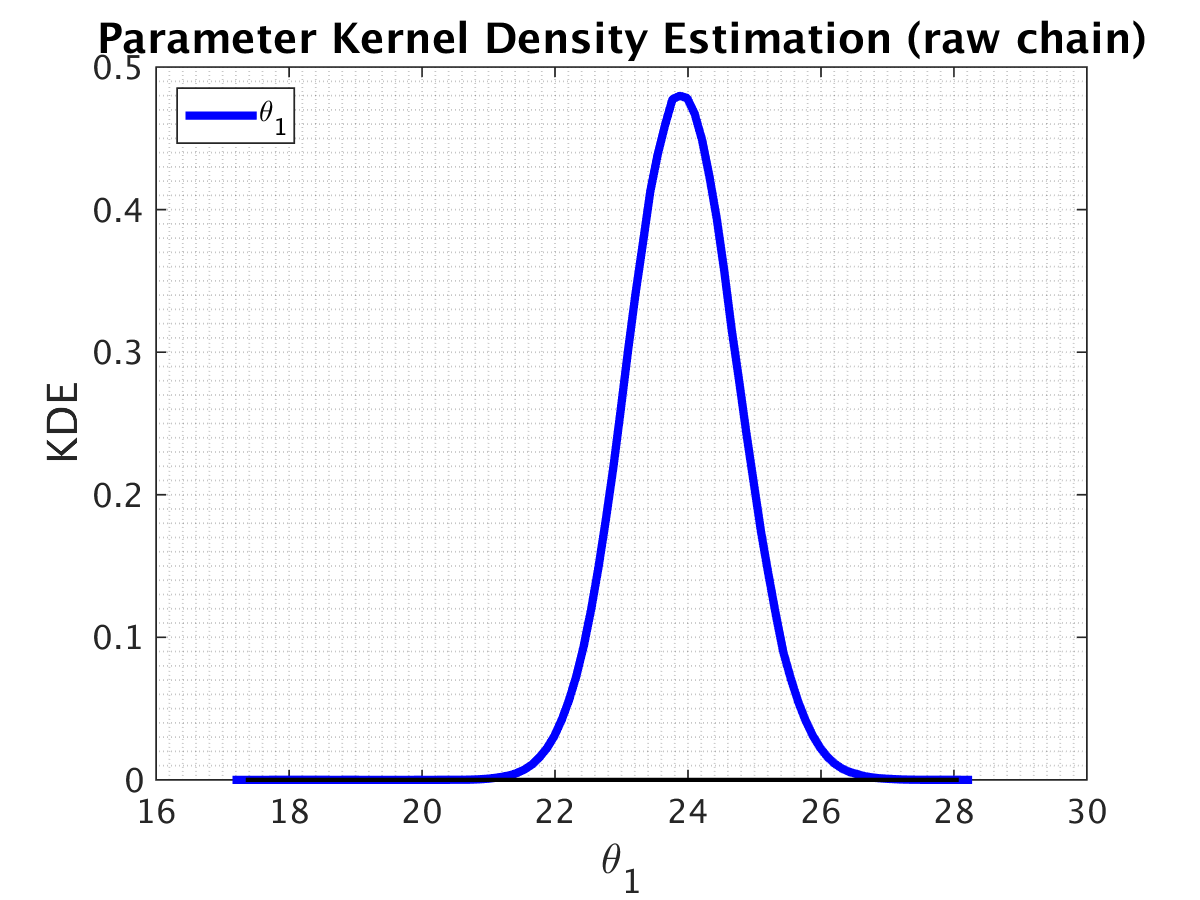
\includegraphics[scale=0.75]{100_results/outputData_900000/simple_ip_kde_raw}
   \caption{ KDE }
\end{figure}

\begin{figure}[H]
  
  \centering
   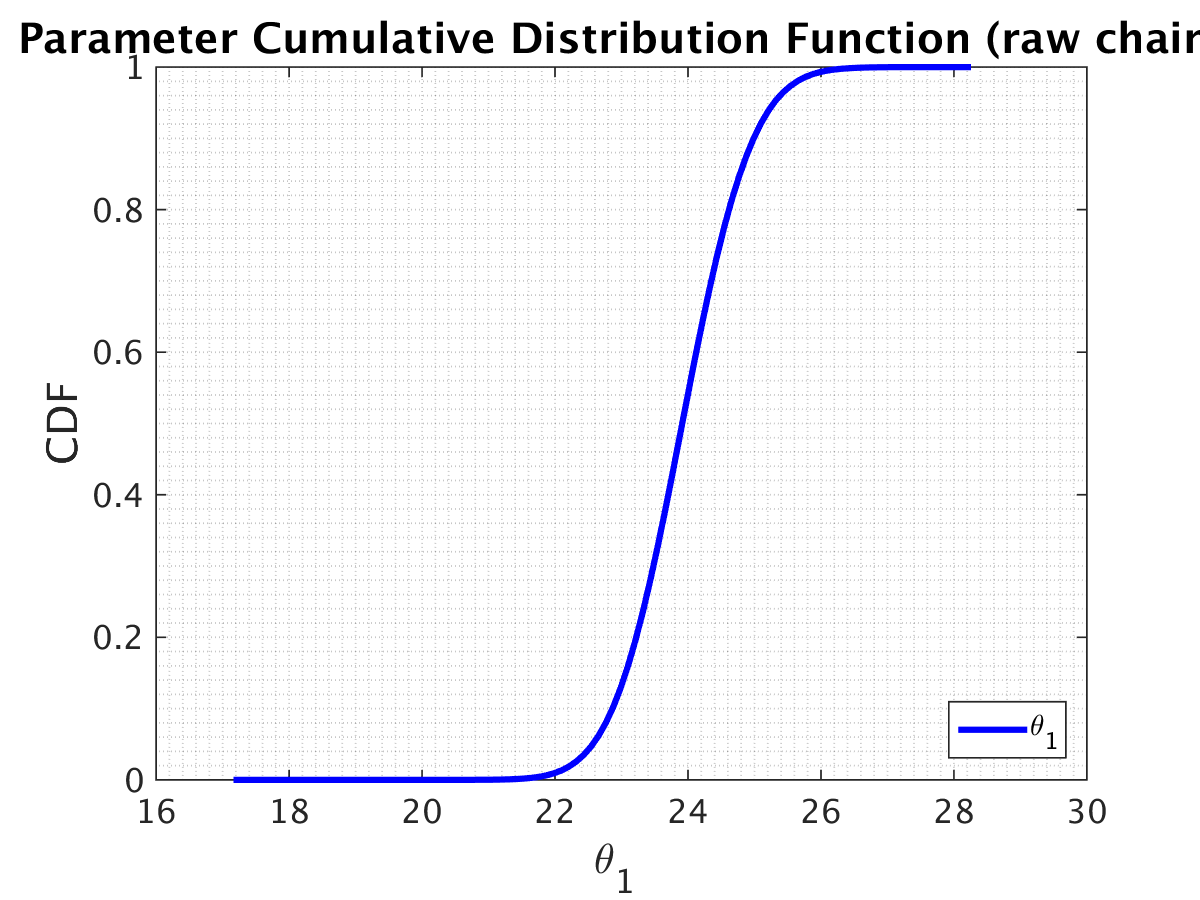
\includegraphics[scale=0.75]{100_results/outputData_900000/simple_ip_cdf_raw}
   \caption{CDF function for Parameter }
\end{figure}



\begin{figure}[H]
  
  \centering
   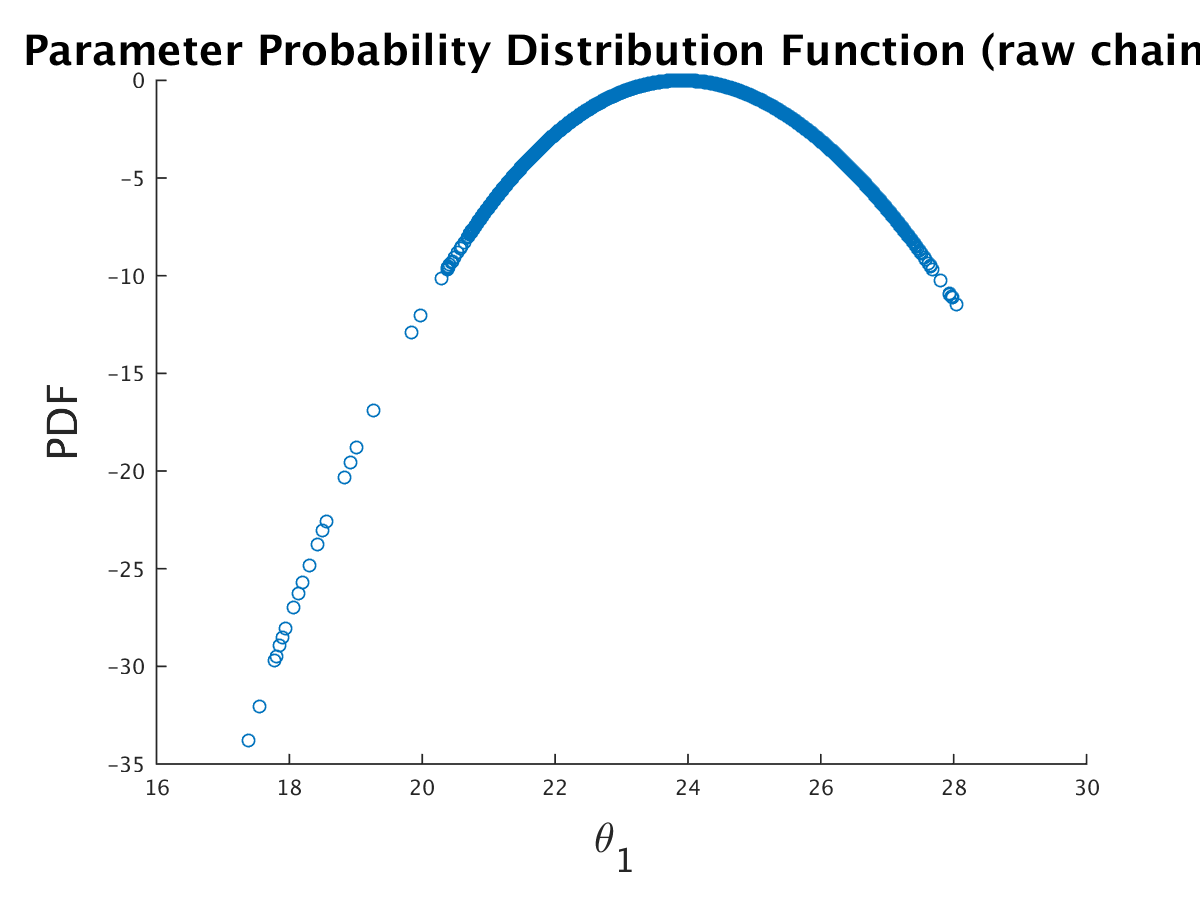
\includegraphics[scale=0.75]{100_results/outputData_900000/ip_logLike_unified}
   \caption{PDF function for Parameter }
\end{figure}


\subsubsection{Chain size 1000000 }
In this section we have chain size of 1000000 points. 

\begin{figure}[H]
  
  \centering
   \includegraphics[scale=0.75]{100_results/outputData_1000000/simple_ip_chain_pos_filt}
   \caption{MCMC chain position }
\end{figure}


\begin{figure}[H]
  
  \centering
   \includegraphics[scale=0.75]{100_results/outputData_1000000/simple_ip_hist_raw}
   \caption{Histogram}
\end{figure}



\begin{figure}[H]
  
  \centering
   \includegraphics[scale=0.75]{100_results/outputData_1000000/simple_ip_kde_raw}
   \caption{ KDE }
\end{figure}

\begin{figure}[H]
  
  \centering
   \includegraphics[scale=0.75]{100_results/outputData_1000000/simple_ip_cdf_raw}
   \caption{CDF function for Parameter }
\end{figure}



\begin{figure}[H]
  
  \centering
   \includegraphics[scale=0.75]{100_results/outputData_1000000/ip_logLike_unified}
   \caption{PDF function for Parameter }
\end{figure}

